% This version uses the latex2e styles, not the very ancient 2.09 stuff.
%\documentclass[letterpaper,twocolumn,10pt]{article}
%\usepackage{usenix}
%\usepackage{epsfig,endnotes}

%\documentclass[sigconf]{acmart}
\documentclass[10pt, sigconf]{acmart}
\usepackage{booktabs} % For formal tables



\usepackage{graphicx}
\usepackage{xspace}
\usepackage[english]{babel}
\usepackage{url}
\def\UrlBreaks{\do\/\do-}

\usepackage{multirow}

\usepackage{algorithm}
\usepackage[noend]{algpseudocode}
\usepackage{multicol}
%\usepackage{amsmath}
%\usepackage{amsthm}
%\usepackage{authblk}

\newtheorem{thm}{Theorem}

%\newenvironment{proof}{ \bf Proof: }{  }


%\newtheorem{theorem}[theorem]
%\newcommand\CommentLine[1]{$\triangleright$ \parbox[t]{\dimexpr\linewidth-\algorithmicindent}{#1}}



\long\def\comment#1{}
\newcommand{\para}[1]{\smallskip\noindent {\bf #1}}
\newenvironment{sitemize}{%
  \begin{list}{$\bullet$}{%
    %\setlength{\rightmargin}{\leftmargin}
    \setlength{\itemsep}{0.2cm}%
    \setlength{\leftmargin}{1.5em}%
    \setlength{\topsep}{0pt plus 0pt minus 2pt}%
    \setlength{\parsep}{0.0cm}}%
  }{\end{list}}
\newenvironment{senumerate}{%
   \begin{list}{\arabic{enumi}.}{%
    \setlength\labelwidth{1.5em}%
    \setlength\leftmargin{1.5em}%
    \setlength{\topsep}{0pt plus 0pt minus 2pt}%
    \setlength\itemsep{0.0cm}%
    \usecounter{enumi}}%
  }{\end{list}}



\newcommand{\eNB}{access point~}
\newcommand{\wf}{Wi-Fi\xspace}
\newcommand{\cf}{CellFi\xspace}
\newcommand{\todo}[1]{\textcolor{red}{\textbf{[[#1]]}}}

\newcommand{\idlow}[1]{\mathord{\mathcode`\-="702D\it #1\mathcode`\-="2200}}
\newcommand{\id}[1]{\ensuremath{\idlow{#1}}}



% Copyright
%\setcopyright{none}
%\setcopyright{acmcopyright}
%\setcopyright{acmlicensed}
%\setcopyright{rightsretained}
%\setcopyright{usgov}
%\setcopyright{usgovmixed}
%\setcopyright{cagov}
%\setcopyright{cagovmixed}


% DOI
%\acmDOI{10.475/123_4}

% ISBN
%\acmISBN{123-4567-24-567/08/06}

%Conference
%\acmConference[CoNEXT'17]{ACM Conference on emerging Networking EXperiments and Technologies}{December 2017}{Seoul, South Korea} 
%\acmYear{2017}
%\copyrightyear{2017}

%\acmPrice{15.00}

\settopmatter{printacmref=false} % Removes citation information below abstract
\renewcommand\footnotetextcopyrightpermission[1]{} % removes footnote with conference information in first column
\settopmatter{printfolios=false}
\pagestyle{empty} % removes running headers

\begin{document}


%\title{Towards unlicensed cellular networks \\ \vspace{0.3in} \normalfont Under submission  - Please do not distribute}
\title{Towards unlicensed cellular networks in TV white spaces}

\author{Ghufran Baig}
\orcid{}
\affiliation{%
  \institution{The University of Texas at Austin}
}
%\email{ghufran@cs.utexas.edu}

\author{Dan Alistarh}
\orcid{}
\affiliation{%
  \institution{Microsoft Research}
}
%\email{email@domain.com}

\author{Thomas Karagiannis}
\orcid{}
\affiliation{%
  \institution{Microsoft Research}
}
%\email{thomas.karagiannis@microsoft.com}

\author{Bozidar Radunovic}
\orcid{}
\affiliation{%
  \institution{Microsoft Research}
}
%\email{bozidar@microsoft.com}

\author{Matthew Balkwill}
\orcid{}
\affiliation{%
  \institution{Microsoft Research}
}
%\email{email@domain.com}

\author{Lili Qiu}
\orcid{}
\affiliation{%
  \institution{The University of Texas at Austin}
}
%\email{lili@cs.utexas.edu}

% \author[2]{Ghufran Baig\thanks{Work performed while an intern with Microsoft Research}}
% \author[1]{Dan Alistarh}
% \author[1]{Thomas Karagiannis}
% \author[1]{Bozidar Radunovic}
% \author[1]{Matthew Balkwill}
% \author[2]{Lili Qiu}
% \affil[1]{Microsoft Research}
% \affil[2]{The University of Texas at Austin}

\begin{abstract}

Unlicensed wireless access is mainstream today, with its prime example, \wf carrying more than 70\% of wireless traffic. 
Unplanned, low-cost deployment and the absence of complex signalling protocols let \wf thrive. 
Yet, \wf and other unlicensed technologies have so far been successful only in short-range scenarios. 
Recently, the availability of TV white space frequencies have promised to extend the benefits of unlicensed networking to long-range scenarios. 
The main technology behind this drive is 802.11af, a \wf variant adapted for TV frequencies, but it has had limited adoption so far.

In this paper we propose \cf, an alternative architecture for cellular networking in unlicensed TV white space frequencies, based on LTE. 
LTE is designed for long-range coverage and throughput efficiency, but it is also designed to operate in tightly controlled and centrally managed networks. 
\cf overcomes these problems by designing an LTE-compatible spectrum database component, mandatory for TV white space networking,
and introducing an interference management component for distributed coordination that requires no explicit communication between LTE base stations. 
Through extensive real world evaluation on off-the-shelf LTE equipment and simulations, 
we show the feasibility of our design and the benefits of \cf compared to 802.11af.






%% \wf is the mainstream wireless access technology today carrying more than 70\% of wireless traffic. 
%% Unplanned, low-cost deployment and the absence of complex signalling protocols let WiFi to thrive. 
%% Yet, WiFi falls short of providing the ubiquitous wireless access and the wide-area coverage demanded by modern cloud-based applications and services. 
%% On the contrary, cellular networks fulfil the goal of coverage at the expense of complex, expensive, and tightly controlled networks that stifle innovation. 

%% In this paper, we design \cf, an unlicensed cellular network that bridges WiFi and cellular technologies. 
%% \cf combines the cheap,unplanned deployment of WiFi with the long-range coverage and throughput efficiency of cellular networks. 
%% To achieve this, \cf is an LTE-based network operating in unlicensed spectrum in TVWS.  
%% To allow for interference management while supporting unplanned deployment, we design mechanisms for distributed coordination that require no explicit communication between LTE base stations. Through extensive simulations and real world experiments on off-the-shelf and custom-built LTE equipment, we show the feasibility of our design and the benefits of \cf compared to existing wireless technologies.
\end{abstract}



\maketitle


%!TEX root = main.tex

%Intro main points:
%\begin{itemize}
%\item Exponential growth on demand for mobile data
%\item WLAN ubiquitous - 70\% of wireless traffic 
%\begin{description}
%\item{+} Uncoordinated
%\item{+} Cheap deployment, infrastucture
%\item{-} Short-range. Coverage is not global (add numbers/measurements)
%\end{description}

%\item Cellular
%\begin{description}
%\item{+} Long-range, broad coverage
%\item{-} Expensive
%\item{-} Proprietary frequency/hardware
%\item{-} Complex ecosystem - stifles innovation
%\item{-} No standards, interoperability in many protocols
%\end{description}

%\item Opportunity: Frequency availability for long-range 
%\item Can we combine the + from WiFi \& Cellular => CellFi

%\item Current options:
%\begin{itemize}
%\item 802.11af - in progress. Problems with range, symmetry, efficiency
%\item 802.22 - unsuccesful, no hardware
%\end{itemize}


%\item Contributions
%\begin{itemize}
%\item CellFi - Long-range unlicenced network
%\item Decentralized algorithm for unccordinated deployment
%\item Measurements in the wild
%\item Complete implementation and simulations
%\end{itemize}


%\end{itemize}

\section{Introduction}
The vision of 5G cellular networks has created exciting new opportunities for innovation. 
While it remains to be seen what technologies will eventually be included in 5G, 
one of the expectations is that
5G will offer greater coverage, capacity improvement, and latency reduction
by leveraging unlicensed spectrum and deploying a large number of
dense access points. Unlicensed spectrum is attractive, as anyone is
allowed to run its network provided a set of agreed rules are respected.  These
rules typically refer to the coordination between technologies and
equipment sharing the spectrum so that use is ``fair.''

The goal of this paper is to design an {\em unlicensed cellular network}, a network which provides cellular-like experience in unlicensed frequencies -- long-range coverage for users with mobile devices,
but at the same time follows the successful model of \wf's unplanned deployment.
To provide coverage, the network should operate in unlicensed spectrum at low UHF frequencies,
taking advantage of the recent availability of frequencies for long-range communications in TV white spaces (TVWS).
The network should meet the regulatory requirements for TVWS~\cite{etsi_tvws, Rice_af} and allow for the deployment of any number of access points without central coordination but with the ability to control mutual interference.

A natural question to ask is \emph{which wireless technology should an unlicensed cellular network be built upon?}
Several standards have been proposed for networking in TV white spaces (802.11af\cite{Rice_af}, 802.22\cite{802.22}, Weightless\cite{weightless}). Most have been abandonded and the TV white spaces efforts now mainly focus 
on 802.11af, which is a modification of Wi-Fi. 
\wf appears as a natural fit for an unplanned deployment in TVWS.
It inherently allows for network co-existence, and 802.11af amendments allow it to operate in TVWS while maintaining its low silicon design cost by significantly reusing existing Wi-Fi design. 
Yet, \wf PHY is not suited for long-range~(Section~\ref{sec:PHY}) and 
\wf's overheads, such as carrier sense and backoff mechanisms, severely limit its efficiency on long range~(Section~\ref{sec:MAC}). 

%Moreover, the asymmetric links between downlink and uplink exacerbate hidden 
%and exposed terminals in long ranges (Section~\ref{sec:PHY}).


Beyond Wi-Fi, another obvious candidate for an unlicenced cellular network could be LTE/4G, which presents a well developed ecosystem for cellular networking in licensed frequency. 
Surprisingly, this option has not been much explored. 
Conventional cellular technologies, such as LTE, are efficient and provide long range~(Section~\ref{sec:PHY}). 
But they are tailored to licensed spectrum where interference is managed either through coordinated control protocols or at deployment phase. 
LTE has no provisioning to avoid primary spectrum users~\cite{etsi_tvws}. 
Further, it has no mechanism to avoid unplanned interference, which can frequently occur in unlicensed bands.
In such cases, current LTE design will lead to significant collisions and performance degradation in TVWS~(Section~\ref{sec:MAC}).  
Further, conventional cellular networks typically represent expensive deployments based on proprietary hardware and software.
Standards and interoperability across protocols and networks are often poorly specified, 
and in general, ``cellular'' reflects a complex ecosystem, tightly controlled by providers and hardware vendors. 
Therefore, LTE in its current form faces major challenges in supporting network co-existence. 


In this paper, we propose {\em \cf}, a TVWS-compliant cellular network architecture built on top of the LTE stack. 
\cf leverages LTE PHY-layer advantages to achieve coverage. 
\cf extends the LTE stack with two new components, a channel selection and an interference management component. 
The channel selection component interfaces with a TVWS database and is able to quickly vacate a channel once it has been assigned to a primary user. 
%The interference management component manages interference among \cf nodes.
Interference management across \cf nodes is based on an algorithm 
 for distributed coordination in LTE that requires no explicit communication or coordination between access points.
The interference management component estimates the number of contending nodes using standard LTE radio mechanisms and uses this estimate to calculate its own network share. Each access point then strategically and independently selects one or multiple LTE resource blocks according to this derived share, 
and relies on the standard LTE scheduler to allocate resource blocks to clients.  

%% Interference is managed through frequency sharing following a two-phase process where
%% channel reservation and resource scheduling are decoupled. Base
%% stations use sensing to conservatively 
%% estimate their fair-share of channels in a distributed fashion. Each base station then strategically selects one or
%% multiple subchannels according to the derived share, 
%% and schedules its clients onto its selected channels. 


To demonstrate the feasibility of \cf and evaluate its performance, 
%we implemented 
%most \cf components on top of off-the-shelf LTE access points. 
we perform several indoor and outdoor experiments as well as large-scale simulations. 
We find that our system can achieve 1km range while maintaining throughput above 1Mbps, and that it can quickly vacate a channel if a primary user appears. 
Moreover, we find that our distributed interference mechanism is effective and in most examined cases better than the one in 802.11af. 
Our contributions can be summarized as follows. 



\begin{sitemize}
\item We demonstrate the limitations
    of the existing WiFi and LTE protocols when deployed in the unlicensed
  cellular scenario. These observations lay the foundation for the  design of \cf.  
\item We develop \cf, a long-range LTE-based, TVWS-compliant cellular architecture with decentralized interference management that allows for unplanned and uncoordinated deployments. 
\item We demonstrate the feasibility of \cf through a series of experiments with off-the-shelf LTE equipment. 
With the exception of interference management component, \cf access points have been operational for several 
months connecting under-privileged users in our local area. Our measurements are further used to guide a large-scale evaluation of \cf. 
\item We show that \cf reduces the number of clients starved due to contention  by 70\%-90\% compared to \wf and LTE. This is achieved without penalizing the total network throughput or application performance.
\end{sitemize}

To our knowledge, \cf is the first attempt to provide an unplanned and uncoordinated LTE-based network in low-frequency unlicensed TVWS spectrum.
Our vision is that \cf is the first step towards reducing the cost and improving the quality of cellular networking, 
while at the same time spurring innovation and new research in a so-far tightly controlled network domain. 




%\section{Motivation}
%\label{sec:motivation}
\section{Requirements for cellular in TVWS}
\label{sec:requirements}

%We start by explaining the requirements of a practical, long-range unlincensed cellular network and 
%examining whether existing technologies can fulfill these requirements. 
%We will focus on Wi-Fi and LTE radio technologies as most of today's high speed wireless networks are based on one of the two wireless standards.
%They incorporate most of the modern PHY and MAC layer design constructs which make them very efficient.
%Wi-Fi variant 802.11af is currently dominant among TVWS hardware platforms whereas LTE dominates the cellular market. 
%Furthermore, well developed designs and accompanying ecosystems make them most viable in business terms. 



\begin{table*}[htb!]
\centering
\begin{tabular}{  c || c | c | c | c || c | c | c  }
   & \multicolumn{4}{c ||}{{\bf PHY} (Section~\ref{sec:PHY})} & \multicolumn{3}{c}{{\bf MAC} (Section~\ref{sec:MAC})} \\ \hline
   %% & \multirow{2}{*}{Design} & Frequency & Coding & 
   %%   Hybrid & \multirow{2}{*}{Access} & \multirow{2}{*}{TX duration} & \multirow{2}{*}{Mode} \\ 
   %% & & chunks & rates & ARQ & & &  \\ \hline
   & {Design} & Freq. chunks & Coding rate & 
     Hybrid ARQ & Access & TX duration & Mode \\ \hline
  {\em 802.11af} & OFDM & 6-8 MHz & $\geq 0.5$ & no & CSMA & up to 4ms & uncoordinated \\ \hline  
  {\em LTE} & OFDMA & 180 kHz & $\geq 0.1$ & yes & Static & 1ms subframes & coordinated 
\end{tabular}
 \caption{Summary of differences between 802.11af and LTE}
  \label{tab:comp}
\vskip -6pt
\end{table*}



Our goal is to design an unlicenced cellular network that comprises the main advantages of the Wi-Fi and cellular. 
Such a network should thus be characterized by wide coverage and be amenable to unplanned deployments. 
We start by examining the requirements of a practical, long-range unlincensed cellular network.


\noindent{\bf Range.} One of the main requirements of an unlicensed cellular network, and its main differentiation against traditional Wi-Fi services is range. 
The TV white space spectrum promises cell range of 1km and above in unlicensed spectrum, as well as better indoor penetration~\cite{Rice_af}. 
We thus require a cell to have a coverage of at least 1km. 
We also require it to have high per-user throughput of at least 1 Mbps, as promised by universal broadband service in many countries~\cite{uni_broadband}.  

\noindent{\bf Database access compliance to unlicenced spectrum.}
The TV White space is currently available for commercial use in the US, Singapore and the UK, and other countries are working on the relevant regulations. 
However, rules for accessing TVWS spectrum bands are different than the ones regulating Wi-Fi bands. 
TVWS spectrum is available to unlicensed devices (secondary users) only in the absence of incumbents (TV and wireless microphones, also called primary users). 
No device is allowed to access the spectrum before checking spectrum availability in a database~\cite{Rice_af}. 
TVWS database compliance is thus an important aspect of the network design.

\noindent{\bf Unplanned deployment in unlicenced spectrum.}
% The other equally important aspect is support for uncoordinated, unplanned deployments. 
To achieve the ease of Wi-Fi deployments, we need support for unplanned, uncoordinated deployments. Since no one owns the spectrum, it is very likely 
that multiple networks will be deployed in the same area and will need to coexist without mandating central coordination, much like Wi-Fi networks coexist today. 

%{\bf BR: Do we want to discuss this or rely on the discussion in \cf section?}
Coexistence between disparate wireless technologies in the same spectrum is a hard challenge, and still not fully solved in practice for many technologies (e.g., Wi-Fi, Zigbee and Bluetooth). In fact, none of the current TVWS standards (802.11af, 802.22 and Weightless) attempts to solve inter-technology coexistence problem. 
\todo{Recently proposed LTE extensions for unlicensed bands (LTE-U) has proposed using of adaptive on/off duty cycle as a mechanism to share the medium with \wf network in unlicensed bands. So effectively in on cycle  only LTE nodes are operational. However LTE-U has no mechanism of sharing spectrum between two interfering LTE nodes during the on cycle.} 
In the same spirit, we will mandate decentralized interference management only among nodes using the same network technology, and assume\todo{ that LTE-U type on/off duty cycling is used for coexistence with \wf }
or in the future, either one technology will prevail or that a database will make sure different technologies will occupy different, non-overlapping parts of spectrum. 



Furthermore, we require our unlicensed cellular design to work entirely in unlicensed spectrum and not require a licensed spectrum anchor, so that anyone, and not only cellular operators, can deploy it. This is in contrast to current LTE proposals for 5 GHz ISM bands \cite{lteuforum_lteu, jian2015coexistence, radisys-lte}. 

%% {\bf Power assymetry}. Finally, an unlicensed cellular network has to cope with power asymmetry. 
%% According to the current TVWS regulation in the US, UK, access points can transmit with powers of up to 4W whereas a client device is limited to a maximum of 100 mW. 
%% However, this asymetry goes beyond regulation, as client devices have far stricter limitations on radiation, heat disspation and battery consumption 
%% (typical cellular phone transmit power is limited to 200mW whereas cell transmit power can go up to tens of Watts). 





%% \subsection{WiFi and LTE preliminaries}
%% \label{sec:prelims}

%% Most of today's high speed wireless networks are based on one of the two wireless standards: LTE and Wi-Fi.  
%% These standards incorporate most of the modern PHY and MAC layer design constructs which make them very efficient.
%% Wi-Fi variant 802.11af is currently dominant among TVWS hardware platforms whereas LTE dominates the cellular market. Furthermore, well developed designs and accompanying ecosystems make them most viable in business terms. 

%% \noindent{\bf Wi-Fi} uses CSMA/CA to avoid interference from other transmitters. 
%% A station checks if the medium is idle for a period of time before each transmission.  
%% If a station detects a collision, implying contention in a network, it extends the idle period. 
%% This allows Wi-Fi to quickly detect and exploit idle channel, but at the same time introduces inefficiencies. 
%% 802.11af PHY is very similar to 802.11ac except that it uses 6MHz and 8MHz channels and works in TVWS frequencies.

%% \noindent{\bf LTE} consists of a set of base-stations and clients, called \emph{eNodeB}s and \emph{UE}s respectively in LTE jargon.  
%% clients share common resources, which are defined in frequency and time in terms of \emph{resource blocks} (RB), each 180 kHz wide and 1ms long. 
%% Both uplink and downlink resource blocks contain signaling, control and data elements spread out in frequency and time. 
%% The signaling elements (reference signals, synchronization signals) are inserted to allow clients to detect LTE transmissions and keep in sync. 
%% The access point is in charge of scheduling both uplink and downlink traffic. 
%% It assigns multiple RBs to various clients and the assignment is communicated over the control channel. 
%% This makes intra-cell LTE communication very efficient. 
%% However, lack of channel sensing limits coordination among neighboring cells.

%% %The data is transmitted in data elements. 


\section{Existing technologies \& unlicenced \\ cellular}
We focus on Wi-Fi and LTE radio technologies as most of today's high speed wireless networks, and in particular cellular and TVWS networks, are based on one of these two wireless standards.
They incorporate most of the modern PHY and MAC layer design constructs which make them very efficient.
%The Wi-Fi variant 802.11af~\cite{Rice_af} is currently dominant among TVWS hardware platforms whereas LTE dominates the cellular market. 
Furthermore, well developed designs and accompanying ecosystems make them most viable in business terms -- client devices with variants of LTE and \wf are available today for under \$50. 



\subsection{Physical layer and coverage}
\label{sec:PHY}


\begin{figure*}[t]
  \begin{minipage}{0.32\textwidth}
    \centering
    (a)
    \vskip -2pt
    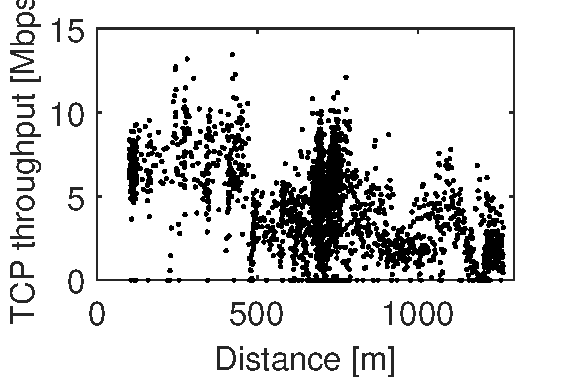
\includegraphics[width=\textwidth]{./figs/range.pdf}
  \end{minipage}
  \begin{minipage}{0.32\textwidth}
    \centering
    (b)
    \vskip -2pt
    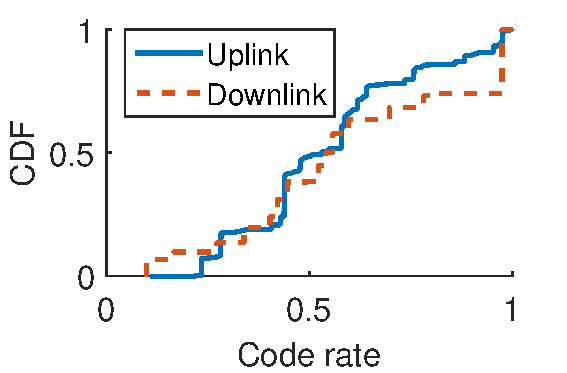
\includegraphics[width=\textwidth]{./figs/coding_rate.pdf}
  \end{minipage}
  \begin{minipage}{0.32\textwidth}
    \centering
    (c)
    \vskip -2pt
    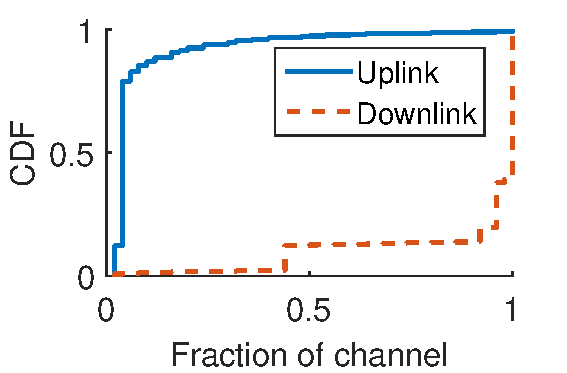
\includegraphics[width=\textwidth]{./figs/NRB.pdf}
  \end{minipage}
 \caption{Throughput as a function of distance (a), CDF of coding rate used (b) and fraction of channel used (c).}
  \label{fig:phy}
\vskip -6pt
\end{figure*}


LTE is based on OFDMA. Its clients share common resources, which are defined in frequency and time in terms of \emph{resource blocks} (RB), each 180 kHz wide and 1ms long. 
Both uplink and downlink resource blocks contain signaling, control and data elements spread out in frequency and time. 
The signaling elements (reference signals, synchronization signals) are inserted to allow clients to detect LTE transmissions and keep in sync. 
LTE PHY is designed for long range, so it contains features useful for low SNR links, such as low coding rates, hybrid ARQ and OFDMA modulation that allows 
the scheduler to use only a subset of resource blocks with the highest signal quality when sending to a specific client.

Most of the LTE hardware already works in a wide range of standardized 3GPP bands~\cite{36_101}. Some of these bands already coincide with TV white space frequencies in parts of the world (e.g., band 44 coincides with part of the TV white space spectrum in the UK). New 3GPP bands are likely to cover even more TV white space spectrum in future (e.g., future LTE bands to cover spectrum sold under US broadcast incentive auctions~\cite{fcc_600}). 
3GPP radio requirements~\cite{36_101, 36_104} adhere to ETSI TVWS spectral mask requirements~\cite{etsi_tvws}. 
Furthermore, the LTE PHY can use a single channel (in TDD mode) and allows for 5MHz, 10MHz, 15MHz and 20MHz bandwidths; it can thus adapt to several contiguous available TV channels (TV channels are 6MHz in the US and 8MHz in the EU). 

Wi-Fi PHY has originally been designed for short range. It uses OFDM, which means that only one client can be served at one time over the entire spectrum, regardless of signal quality on each subcarrier. Newest Wi-Fi standards (802.11ac) use high coding rates, the minimum being 1/2. 
The recent 802.11af~\cite{Rice_af} standard specifies amendments to 802.11 to allow WLAN to operate in the TVWS spectrum. The standard has opted to keep the main features of the 802.11 PHY in order to minimize the cost of modifications. 802.11af PHY uses 6MHz and 8MHz channels and works in TVWS frequencies. It has the same modulation and coding rates as 802.11ac. 

Table~\ref{tab:comp} summarizes the properties of the two technologies. To better understand the impact of these in practice for long-range, we perform an outdoor experiment. We are unable to find 802.11af hardware that operates in the frequencies that we have access to. Instead, we perform an experiment using LTE hardware and monitor the impact of key properties from Table~\ref{tab:comp}, such as OFDMA, coding rate and Hybrid ARQ, on coverage. We deployed an LTE small cell on the top of our building. We moved a client throughout the coverage area and recorded its location, the downlink TCP rate achieved using iperf and various LTE performance metrics (please see Section~\ref{sec:implementation} for a detailed description of this experiment). 

Figure~\ref{fig:phy} presents the results of the experiment. 
We observe that with 36dBm EIRP (29dBm transmit power and 6dBi directional antenna) at the AP and 20dBm transmit power at the client (maximum according to TVWS specs), LTE can reach 1.3km in the urban environment.
We measured and achieve 1Mbps TCP rates at more than 85\% of measured locations (in Figure~\ref{fig:phy}(a)). 
In order to achieve these ranges LTE frequently used very low coding rates (Figure~\ref{fig:phy}(b)). 
In fact, the median coding rate was 1/2, which corresponds to the lowest coding rate offered by 802.11af~\cite{Rice_af}. 
Further, LTE leverages its OFDMA capabilities and schedules  
uplink transmission consisting solely of TCP ACK packages which are small in size
in a single resource block. This is shown in Figure~\ref{fig:phy}(c), where we plot the CDF of the fraction of the channel used by transmissions.
LTE chooses the resource block with the highest signal strength and improves the quality of transmission -- this also explains why the LTE uplink and downlink used similar coding rates. 
In similar scenarios, WiFi would reduce the signal quality and consequently the range of the network, 
since it does not implement OFDMA and it would have to send uplink packets across the entire bandwidth. 
Finally, we observe that LTE leverages hybrid ARQ to improve communication quality, and in particular for longer links - we see that 25\% of packets sent from distances larger than 500m use hybrid ARQ. 

%Wi-Fi does not implement OFDMA and it will have to send uplink packets across the entire bandwidth, which will reduce the signal quality and consequently the range of the network. 

%In order to compare the performance of the two PHYs, , and evaluated its performance outdoors. 
%The results are depicted in Figure~\ref{fig:phy}. We were unable to get an 802.11af hardware at the time. Instead we look at the results of our experiments and compare with the main design point of 802.11af (see Table~\ref{tab:comp} for head-to-head comparison). %

%Secondly,, 

%Thirdly,. Uplink transmission consisted solely of TCP ack packages which are small in size, and LTE was able to leverage its OFDMA capabilities and schedule it in a single resource block. Consequently, it is also able to choose the resource block with the highest signal strength and improve the quality of transmission (which also explains why LTE uplink and downlink used similar coding rates). Wi-Fi does not implement OFDMA and it will have to send uplink packets across the entire bandwidth, which will reduce the signal quality and consequently the range of the network. 
%Finally, we observe that LTE leverages hybrid ARQ to improve communication quality, and in particular for longer links - we see that 25\% of packets sent from distances larger than 500m use hybrid ARQ. 

Overall, we see that the unique features of the LTE physical layer (as shown in Table~\ref{tab:comp}), namely, 
low coding rates, OFDMA medium access, and hybrid ARQ play a significant role in the LTE link quality and its ability to provide coverage of 1km and beyond. 



\subsection{Medium access and interference}
\label{sec:MAC}


%% \begin{figure}[t]
%%   \centering
%%     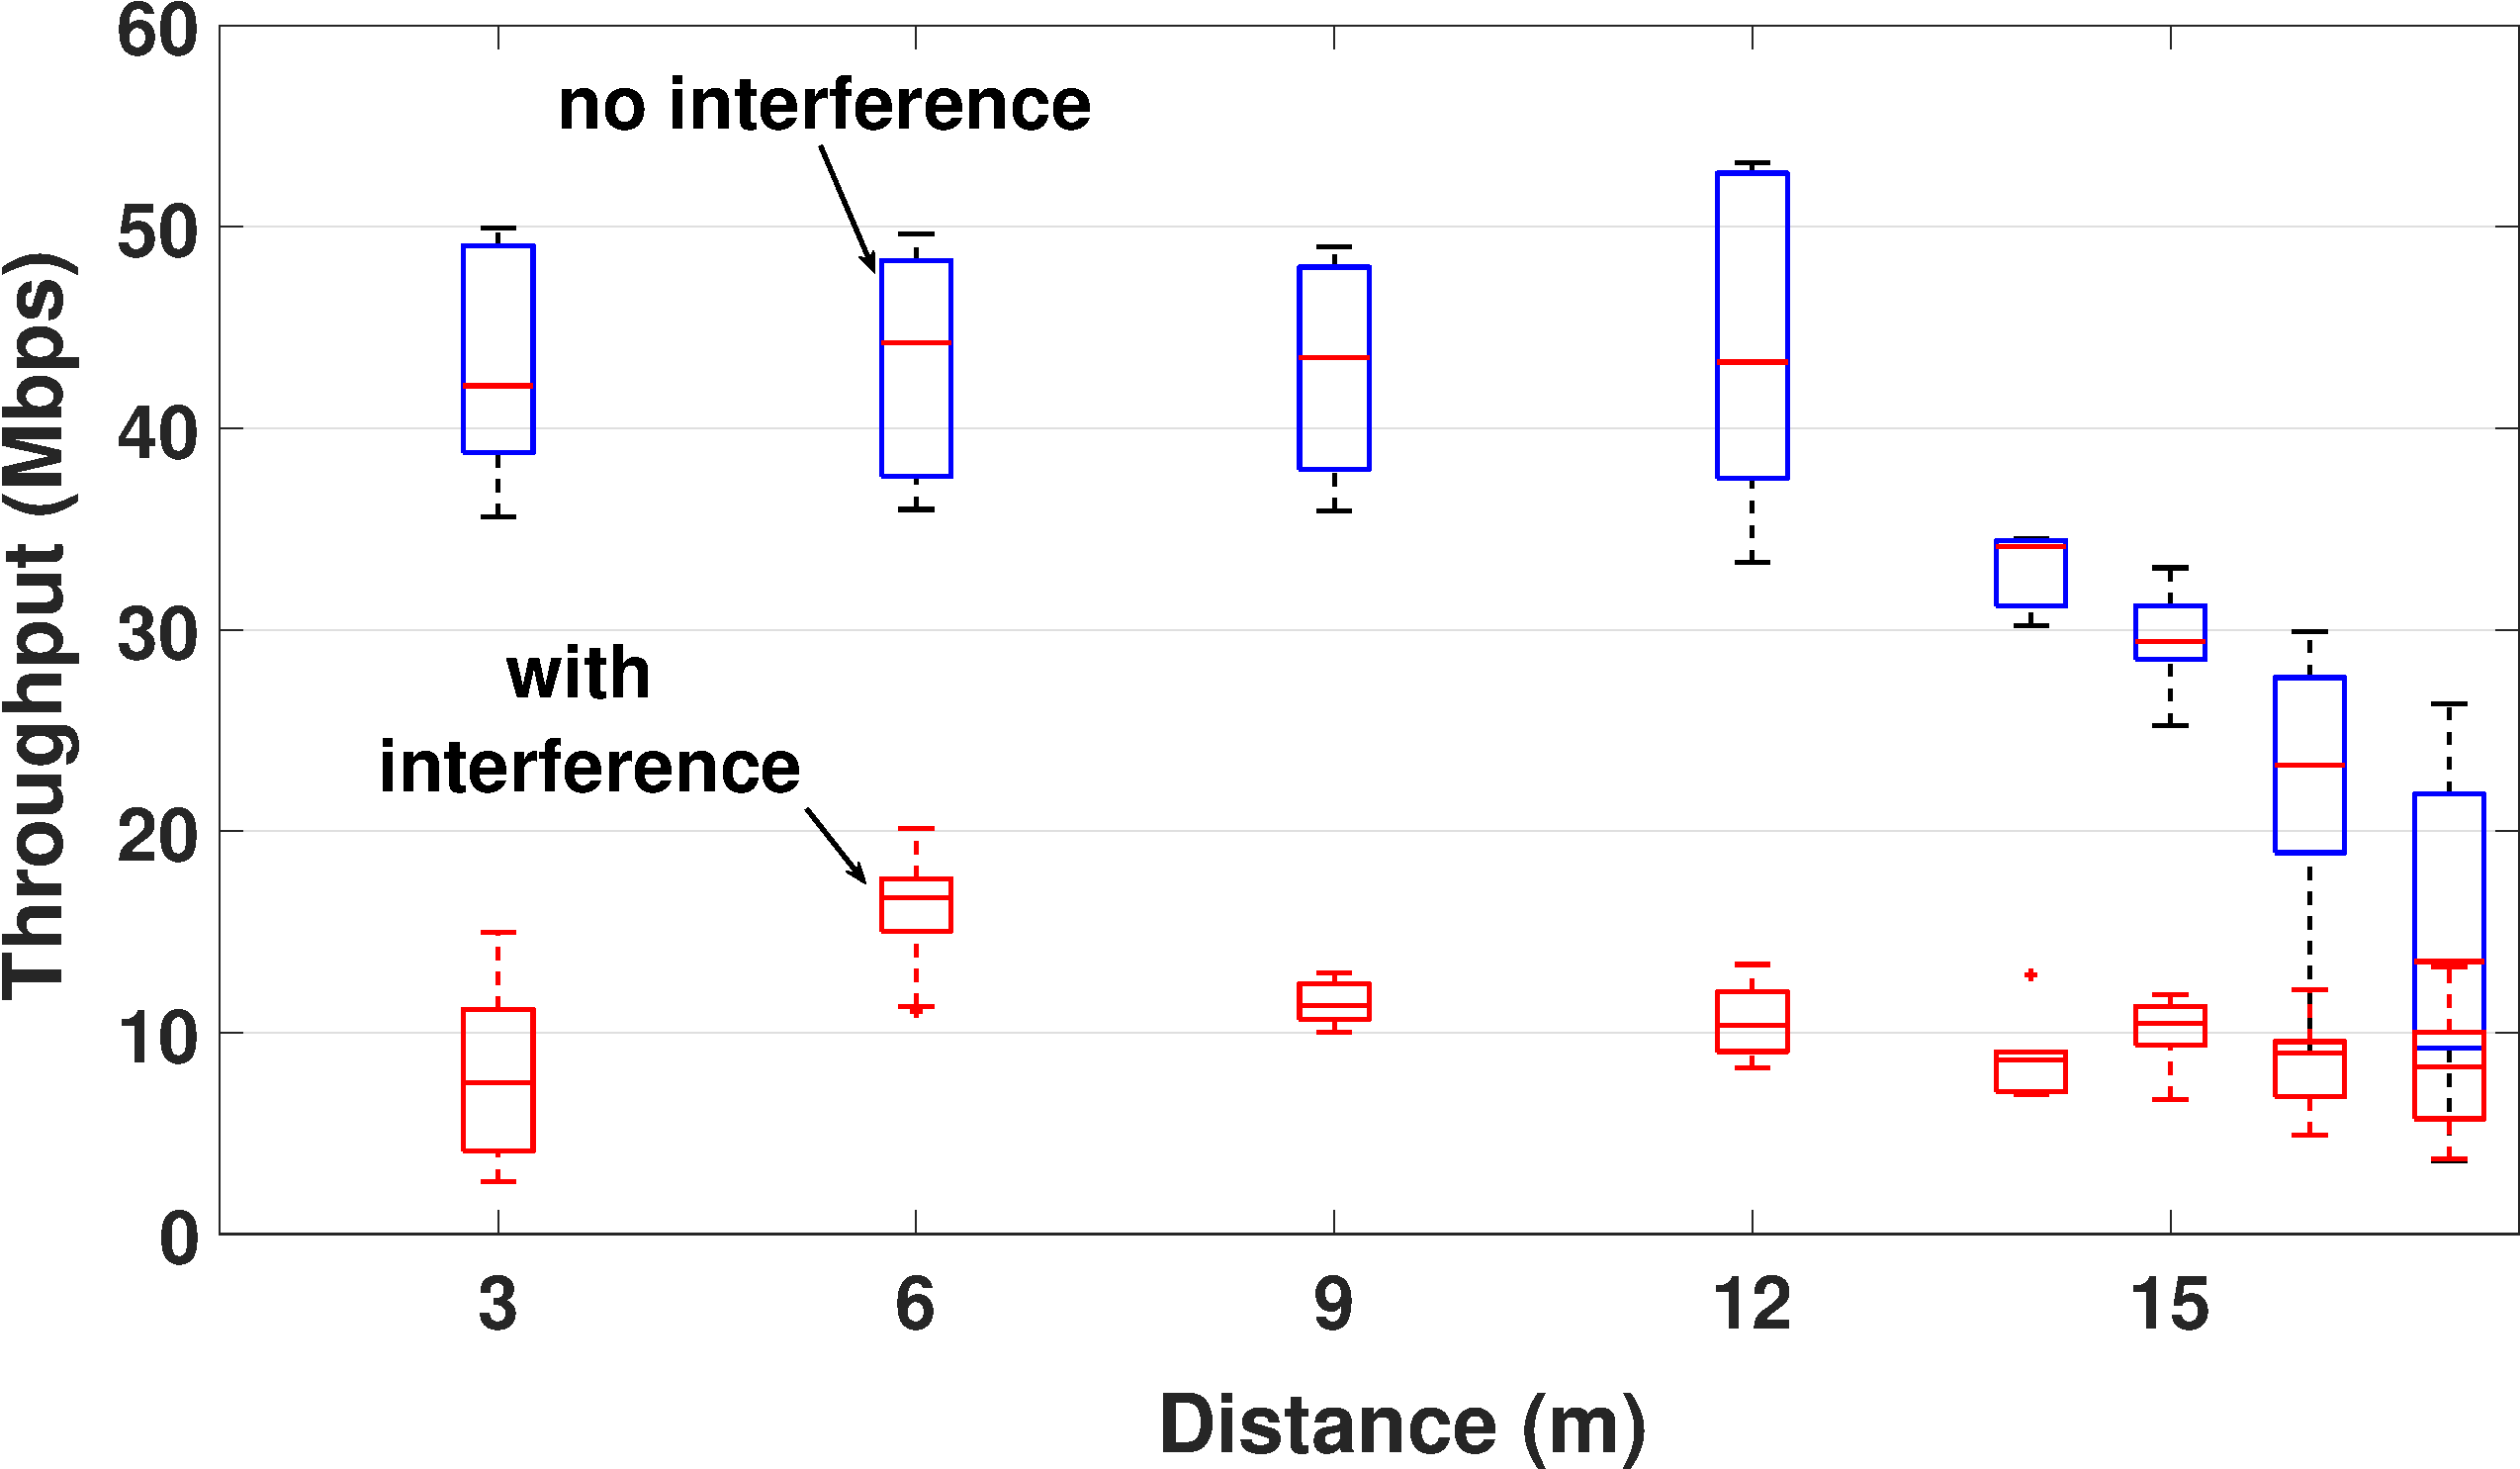
\includegraphics[width=0.5\textwidth, height=0.5\columnwidth]{./figs/interf_data-crop.pdf}
%%     \vspace{-0.3in}
%%   \caption{Throughput of a client with and without interference from an interfering access point. 
%%     The \emph{x-axis} refers to the distance from the serving access point.}
%%   \label{fig:interf}
%% \end{figure}


In LTE, an access point is in charge of scheduling both uplink and downlink traffic. 
It assigns multiple resource blocks to various clients and the assignment is communicated over the control channel. 
This makes intra-cell LTE communication very efficient. 
LTE assumes no unexpected interference from other networks; 
LTE deployments are well-planned and placement and configuration of access points is such that interference is managed in a coordinated fashion, 
either from a central network controller or through explicit coordination between neighbouring access points
(e.g., through X2 protocols~\cite{36_423}).

In an unlicensed band, these assumptions no longer holds true, as we can witness in numerous unplanned Wi-Fi deployments whose owners make no effort to optimize them. 
Regulators have also stirred clear from using a TVWS spectrum database to manage interference between unlicensed, secondary users. 
LTE offers no mechanisms to mitigate interference in uncoordinated deployments, where interference can significantly reduce performance. 
We illustrate this in detail in an experiment described in Figure~\ref{fig:interf_control} in Section~\ref{sec:interfeval},
where we show that a strong interferer (with SINR $\leq 10$ dB) can degrade LTE throughput by up to $2\times$, and also cause frequent disconnections. 
Thus, in order to make unplanned LTE deployment efficient, one needs to manage interference. 

\todo{There have been recently proposed LTE extensions for unlicensed bands (LTE-U/LAA) that try to mitigate interference between neighboring base stations. However LTE-U focuses only on coexistence between LTE and WiFi. It proposes Carrier Sense Adaptive Transmission (CSAT) to efficiently co-exist with WiFi but does not tackle the issue of coexistence of two separate LTE networks. LAA has proposed a contention protocol similar to WiFi CSMA to medium access. This enables LAA networks to coexist with both WiFi and other LAA networks, however its performance will suffer in long range whitespace networks as it will face similar MAC inefficiencies as 802.11af since the medium access mechanism is similar in both technologies.}


%% \begin{figure}[t]
%%   \centering
%%     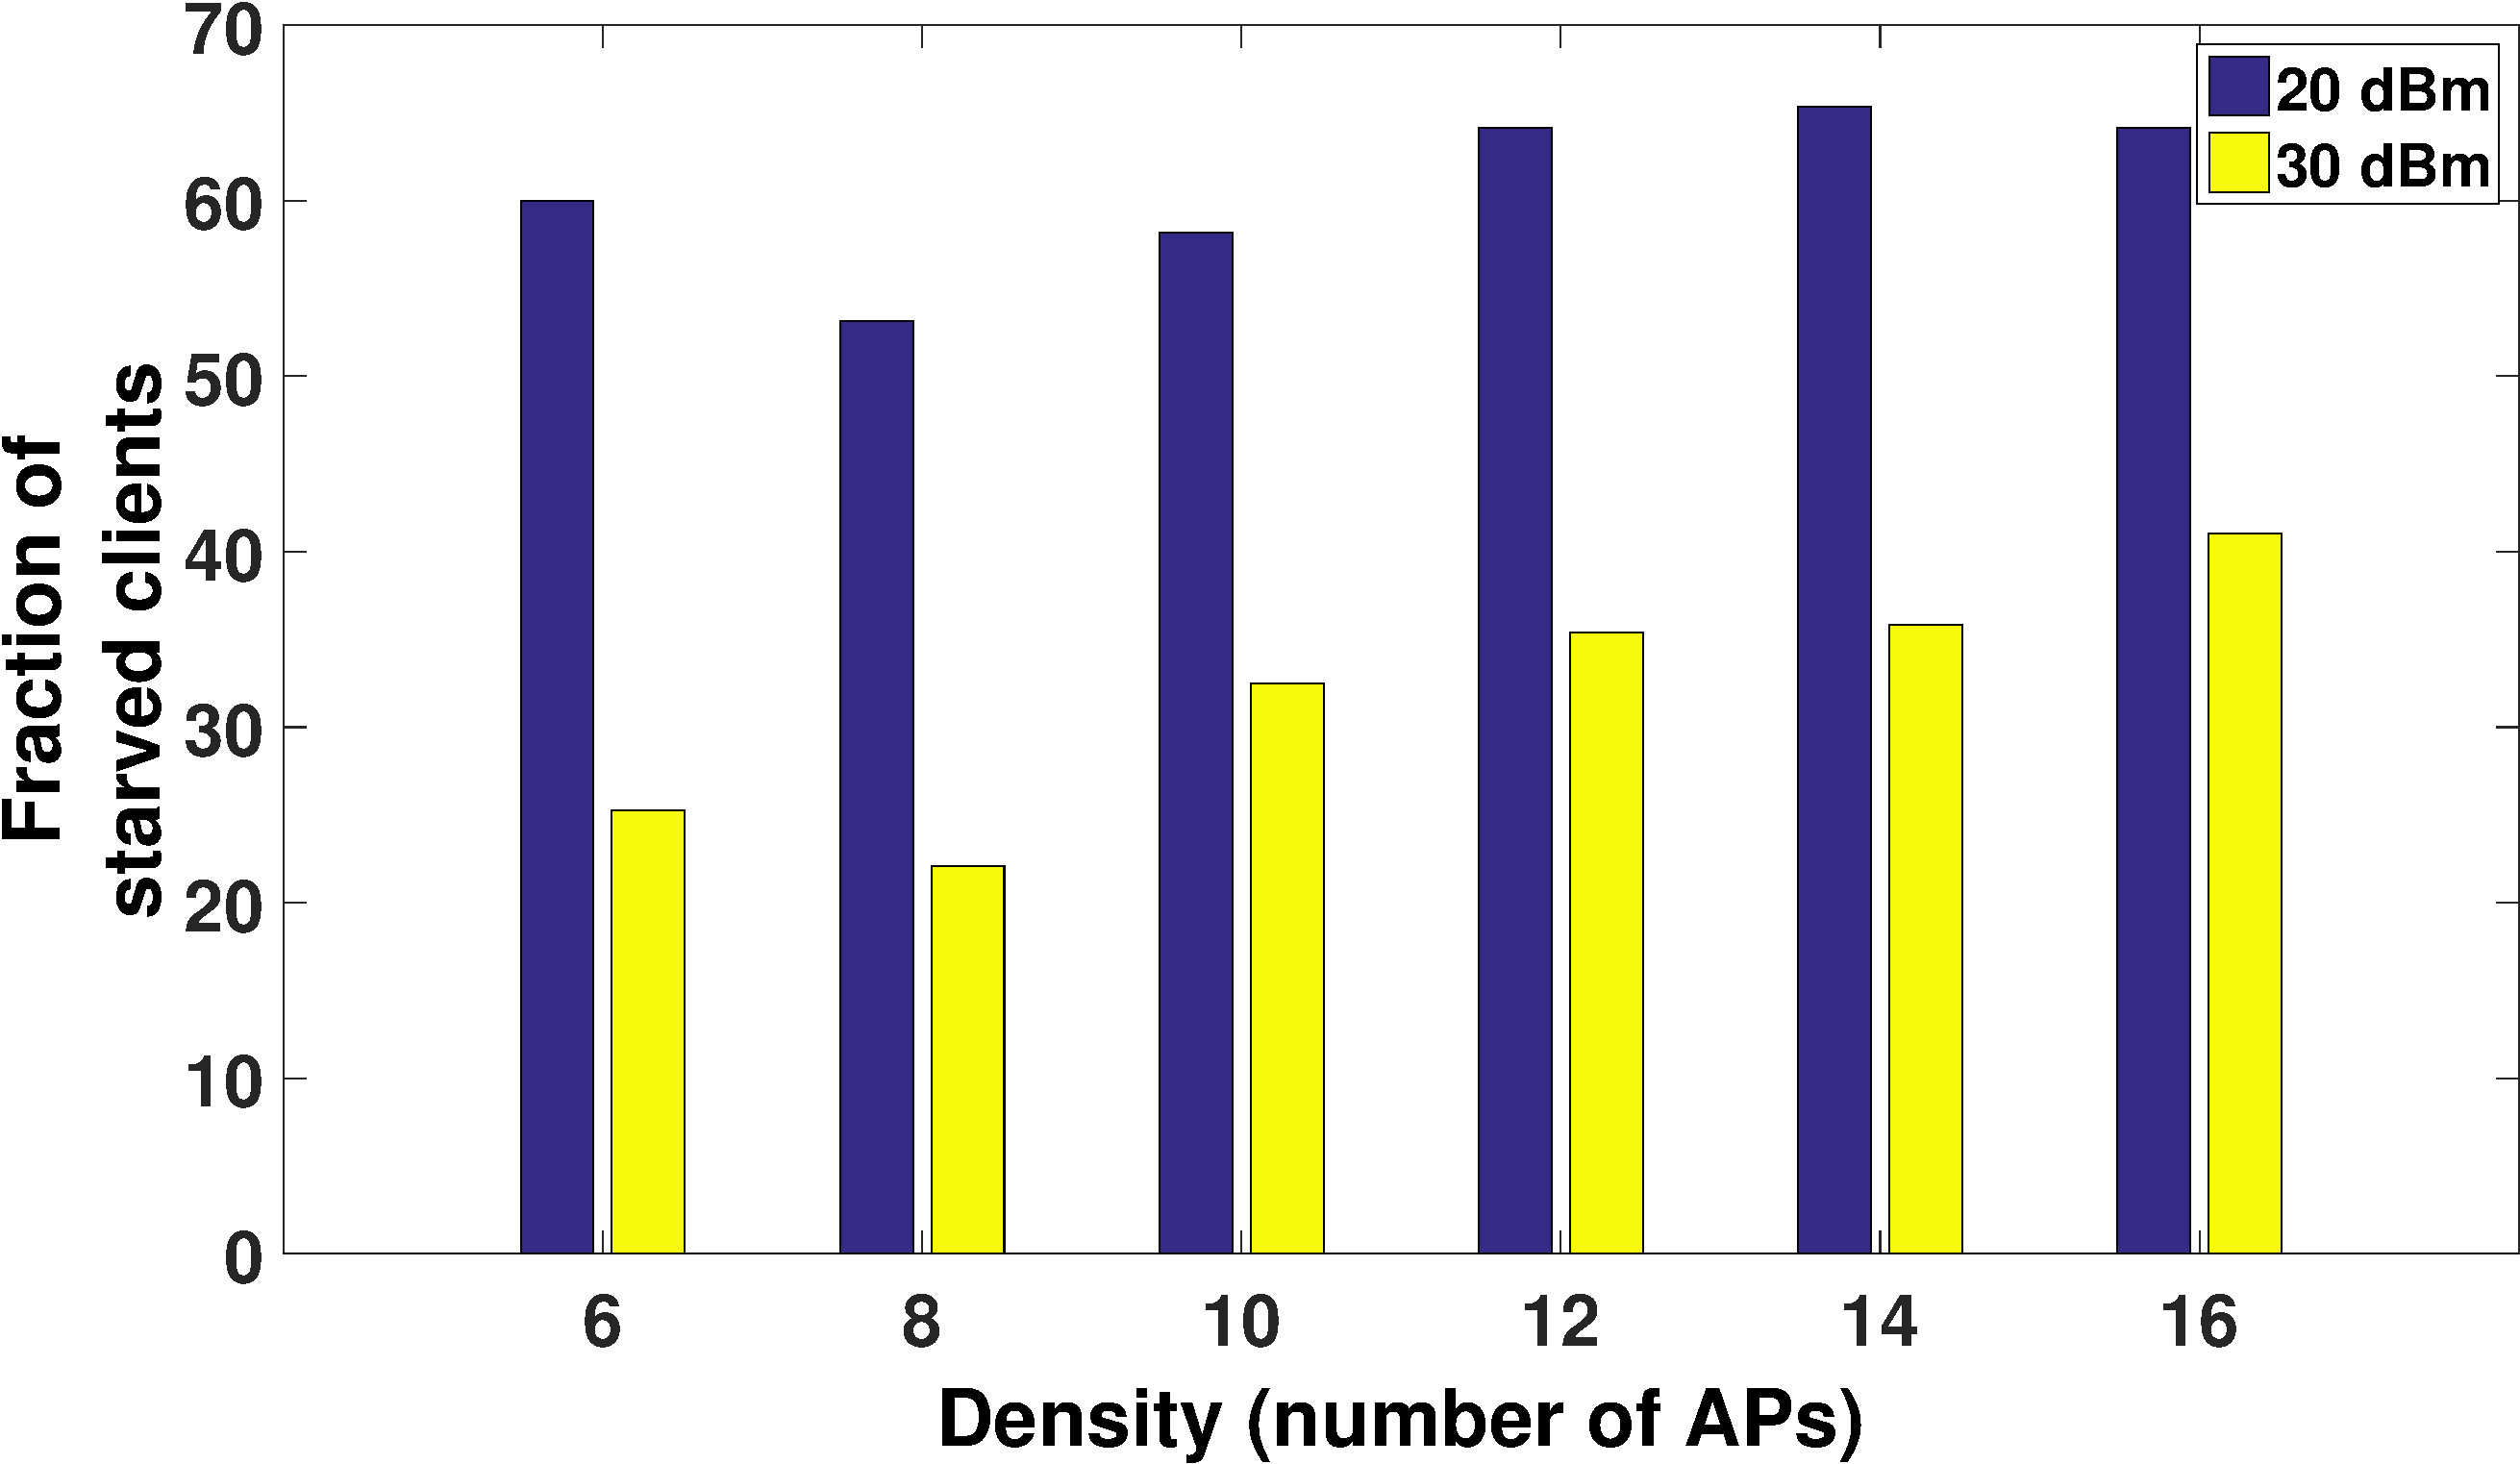
\includegraphics[width=\columnwidth, height=0.4\columnwidth]{./figs/WiFiComparison-crop}
%%     \vspace{-0.3in}
%%   \caption{Fraction of starved clients in a 802.11af deployment for different client transmit powers.}
%%   \label{fig:starved}
%% %\vspace{-36pt}
%% \end{figure}

\begin{figure}[t]
  \centering
    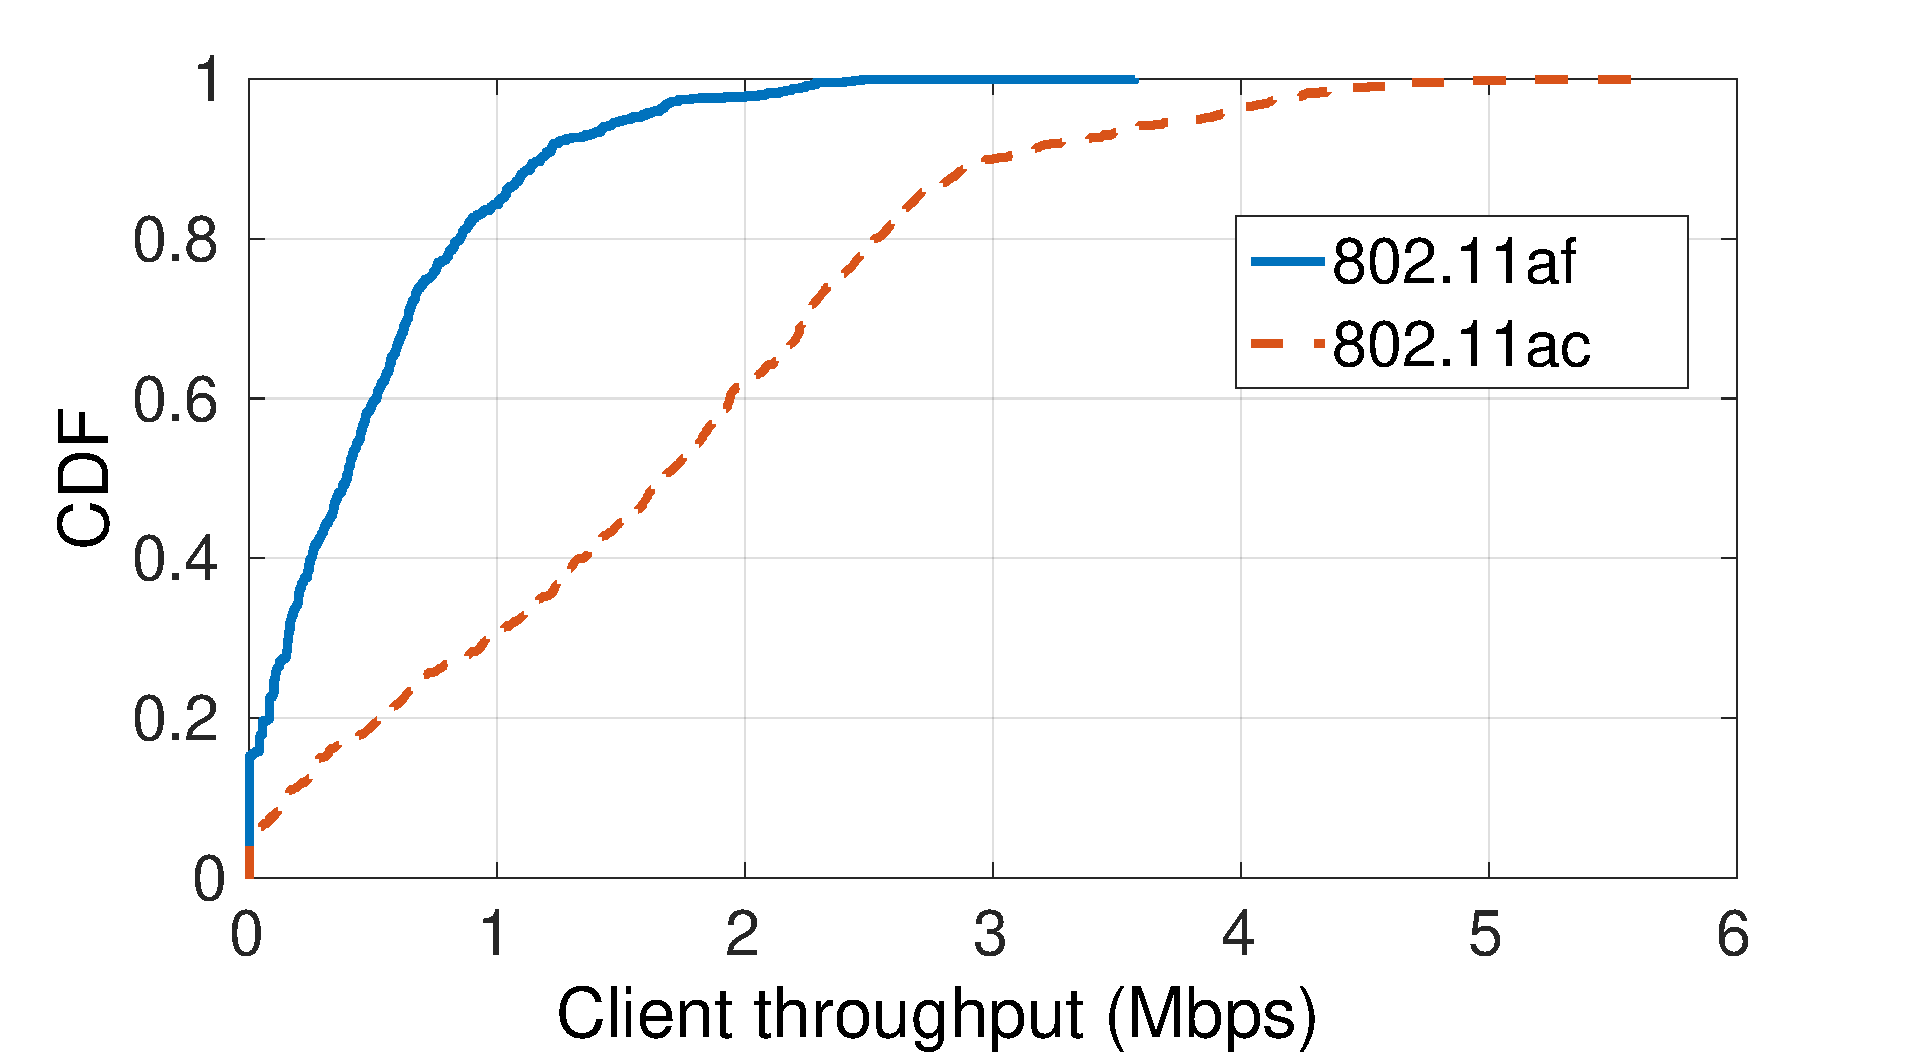
\includegraphics[width=\columnwidth, height=0.4\columnwidth]{./figs/af_vs_ac.pdf}
    \vspace{-0.3in}
  \caption{Wi-Fi MAC inefficiencies.}
  \label{fig:inefficiencies}
\vskip -8pt
\end{figure}



The 802.11af~\cite{Rice_af} standard inherits CSMA medium access mechanism from Wi-Fi, making it suitable for unplanned deployment. 
CSMA is able to use a channel whenever it is available, and quickly back off and adapt once other users are present. 

However, a number of well-known issues in \wf design render its deployment in TVWS problematic, such as hidden and exposed terminals and scheduling efficiency and fairness~\cite{idle_sense}.
These issues are even more pronounced in a long-range network. To illustrate this, we simulate 802.11af and 802.11ac networks in ns3 (please see Section~\ref{sec:eval} for details of simulation settings). 
In both cases we use 20 MHz channels, and we use RTS/CTS as we have observed that it improves performance. 
In both cases we consider the same network of access points and place the same number of clients within the corresponding range of each access point. 
The network range is smaller in case of 802.11ac (home Wi-Fi) than 802.11af (outdoor cellular) because of lower power (20dBm vs 36dBm) and worse propagation, 
but the average SNR at the receiver is same in both scenarios. 
However, the throughput of the 802.11af networks is much worse, as can be seen in Figure~\ref{fig:inefficiencies}.
Therefore, although CSMA offers efficient and fair contention resolution in shot-range Wi-Fi networks, this is far from obvious in the cellular scenario. \\

{\bf Summary.} Overall, LTE appears as a better fit for a TV white space cellular network due to its unique PHY and MAC layer properties.
However, it has never been fully considered as a candidate design due to its lack of uncoordinated interference management. We explore this by describing \cf over the next sections.




%% As already discussed, the links in TVWS networks are asymmetric, with APs transmitting at 30dBm power and mobiles
%% transmitting at 20dBm power, which significantly degrades carrier sensing. 
%% This is shown in Figure~\ref{fig:starved}, which shows
%% the fraction of starved clients for \wf in TVWS. The details of this experiment
%% can be found in Section~\ref{sec:eval}. 
%% The figure also reminds us that exposed and hidden terminal
%% inefficiencies are still present even when clients and APs use the
%% same transmit power (30 dBm in this example).




%% {\bf Ghufran, Lili: Write more about what are the reasons for poor WiFi's behaviour.}
%% \begin{figure}[t]
%%   \centering
%%     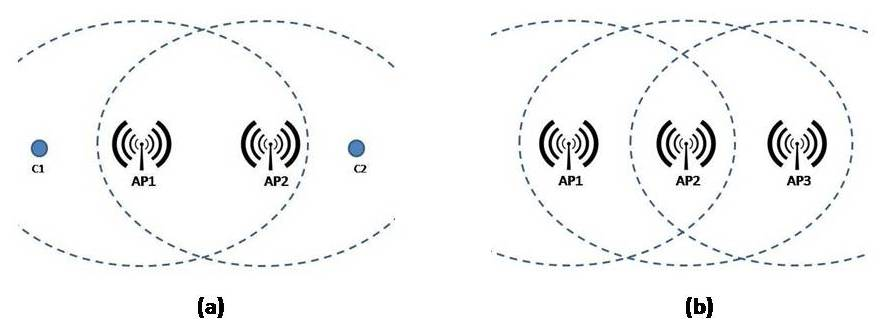
\includegraphics[width=\columnwidth, height=0.4\columnwidth]{./figs/wifi_inefficiencies.jpg}
%%     \vspace{-0.3in}
%%   \caption{CSMA inefficiencies.}
%%   \label{fig:inefficiencies}
%% %\vspace{-36pt}
%% \end{figure}
%% \begin{itemize}
%% \item {\bf Issues in uplink vs. downlink}\\
%% Figure~\ref{fig:inefficiencies} (a) shows an example in which AP1 is prevented from sending packets to its client (C1) because neighboring AP2 is transmitting to its client (C2). Ideally both APs should be able to send simultaneous downlink transmissions but Wi-Fi CSMA causes AP1 to conclude that it will interfere with the transmission by its neighbor AP2, However C1 can still receive the transmission of AP1 without interference because it is out of range of AP2. The primary reason for this issue is that for a downlink transmission the CSMA is done on the uplink instead. The simulation results for the scenario depicted in the figure show that this issue causes the total network throughput to be effectively halved of what it ideally should be.\\
%% \item { \bf Issues in multiple downlinks}\\
%% Wi-Fi guarantees an equal long term channel access probability to all hosts. This causes the throughput of all clients with higher bitrate to be reduced to the throughput of the client with lowest bit rate because The slower client gets a higher air time compared to the faster client, resulting in unfair resource allocation and overall throughput degradation of the network.
%% \item {\bf Issues in multiple APs}\\
%% Figure~\ref{fig:inefficiencies} (b) shows an example in which AP2 interferes with both AP1 and AP3, but AP1 and AP3 can not listen to each other's transmissions. In this scenario Wi-Fi CSMA would cause AP2 to starve if AP1 and AP2 do not transmit in a perfectly synchronized manner. This is because both AP1 and AP3 can transmit simultaneously and unless their transmissions end at the same time AP2 would always find the channel busy. The simulations results for the scenario depicted in the Figure show that AP2 manages to get an airtime of only around 3\% whereas AP1 and AP3 keep transmitting for the rest of the time.\\ 
%% \end{itemize}





%% \subsection{Towards an ideal design}
%% \label{sec:ideal}

%% In summary, both Wi-Fi and LTE have its deficiencies when applied to unlicensed cellular scenario in TV white spaces. 
%% However, LTE seems a better candidate yet it is rarely considered as a candidate design for TV white spaces. 
%% Wi-Fi design is inadequate for both PHY and MAC. 
%% LTE's PHY is well suited for long range and high bandiwidth. 
%% We next argue that LTE MAC and network layers can be adapted, with software modifications, to meet the other requirements of TV white space networking, such as decentralized interference management and channel selection through the database.




\section{\cf}

%As we have seen from the previous discussion, LTE seems potentially a better technology for TV white space, yet it has never been fully considered as a candidate design. 

\cf enables long-range, unlicenced networking in TV white spaces 
%is an architecture for TV white space networking 
based on the LTE stack. \cf incorporates software-based adaptations on the LTE stack to be compliant with
 requirements of TV white space spectrum access, such as avoiding primary users through a spectrum database, and incorporates decentralized interference management to cater for unplanned deployments. 
This section provides an overview of the \cf architecture and its basic building blocks.

%we explore this option and propose \cf, a novel architecture for TV white space networking based on LTE stack, adapted with software modifications to meet the requirements of TV white space spectrum access, such as channel selection through the spectrum database and decentralized interference management.


\subsection{Overview}

\cf is built on the top of standard LTE network architecture. It consists of small cell access points, mobile clients and an LTE control plane (EPC). It also includes a standard TV white space database. Figure~\ref{fig:arch} presents an overview of the \cf architecture.

%The \cf access point consists of three components. 
Compared to the traditional LTE, the \cf access point introduces two new software components, namely interference management and channel selection, and it is equipped with a GPS.
The channel selection is responsible for maintaining a list of available channels from a spectrum database and selecting the most appropriate one. 
The intra-channel interference management component decides which resource blocks within the channel can be used by the access point and which should be left for others, 
depending on the demand observed for the same channel. The GPS is introduced for two reasons. First, a GPS is required for any TV white space system to provide an accurate location to the spectrum database~\cite{Rice_af}. 
Second, \cf uses TDD LTE allowing it to use a single channel for both downlink and uplink and thus have more flexibility when choosing available spectrum. A GPS clock is indispensable for TDD LTE in order to synchronize interfering uplink and downlink transmissions across multiple networks. Finally, the access point contains the standard LTE small cell software stack that communicates with the control plane (EPC), 
schedules data packets, etc. 


% \cf access point is equiped with a GPS, for two reasons. Firstly, a GPS is required for any TV white space system to provide an accurate location to the spectrum database. Secondly, \cf uses TDD LTE allowing it to use a single channel for both downlink and uplink and thus have more flexibility when choosing available spectrum. A GPS clock is indispensable for TDD LTE in order to synchronize interfering uplink and downlink transmissions across multiple networks. 


\begin{figure}[htb]
  \centering
    \vspace{-12pt}
    %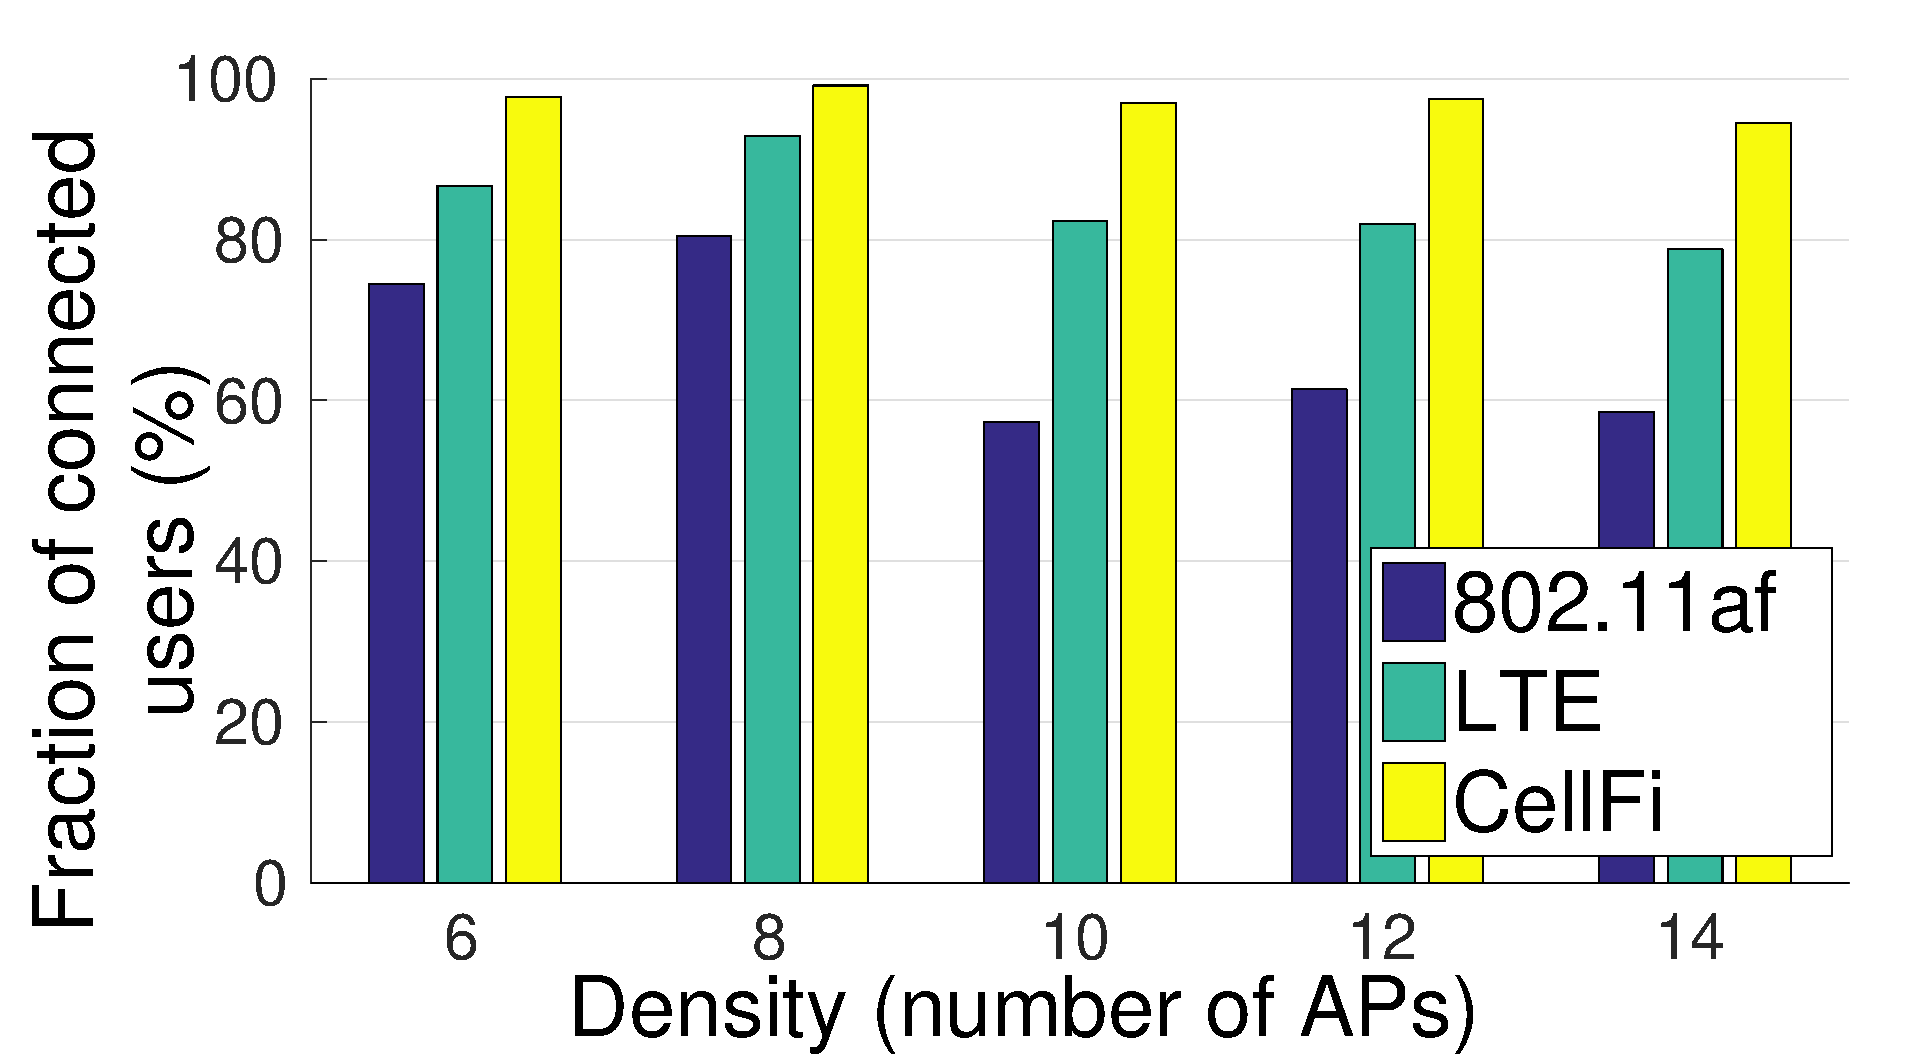
\includegraphics[width=\columnwidth, height=0.38\columnwidth]{./figs/density-crop}
    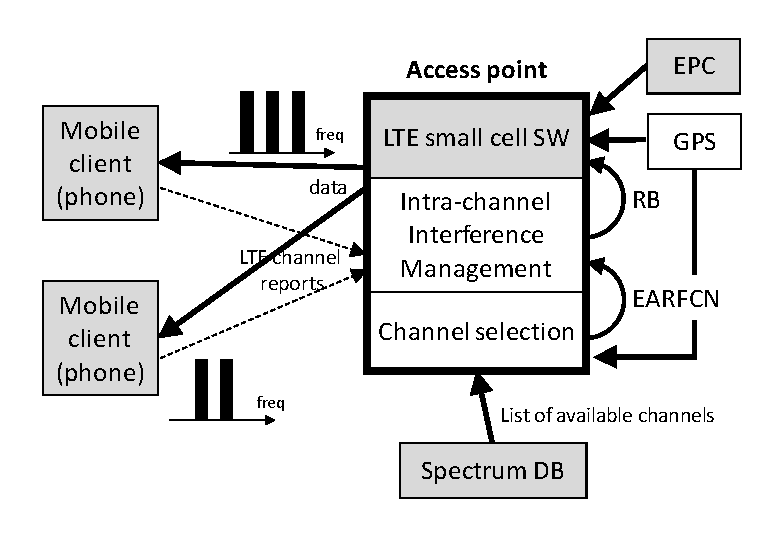
\includegraphics[width=\columnwidth]{./figs/architecture}
    \vspace{-0.3in}
    \caption{\cf architecture overview. The shaded blocks denote unmodified existing components (parts of LTE network stack and TVWS database) and the white blocks are new components introduced by \cf. }
  \label{fig:arch}
\end{figure}

%TWe implement the two new components (interference management and database client) in software. We next explain in detail each of the components and how they interface with the rest of the system.  



\subsection{Channel Selection}

Spectrum access in TV white spaces is managed through a spectrum database~\cite{fcc_db, ofcom_db}. 
The TVWS client in the \cf access point operates by sending the GPS location details to a TVWS database server~\cite{paws},
to which the database responds with a list of available channels (if any), how long then can be used and maximum allowed power levels.  
%There are two types of TVWS client : (i) master client, which in LTE is the access point, and (ii) slave client(s), which in LTE are the mobile devices.
No TVWS client is allowed to transmit in a channel without having a valid lease from a spectrum database and has to stop once a lease has expired.

Satisfying these rules is not straightforward in general. Consider a Wi-Fi client that has associated itself to an AP on a channel with a valid spectrum lease and has gone to sleep. 
In order to be compliant, the client needs to verify the validity of the channel before accessing it next time it has a packet to send, which requires changes to the standard Wi-Fi architecture. 
On the other hand, LTE architecture lends itself to this type of requirements. An LTE client has to get a grant for each uplink transmission from its access point. 
Thus, once an access point looses a spectrum lease and stops transmitting, all of its clients will stop transmitting instantly 
(we demonstrate this in practice for \cf in Section~\ref{sec:database-eval}).

%Furthermore, an LTE access point will only transmit if it has an open SCTP connection to the LTE control plane (EPC). Once this connection is down, the access point will switch the radio off. 

We leverage this observation and build an ETSI-compliant~\cite{etsi_tvws} TVWS database client using the PAWS protocol~\cite{paws}. 
In our architecture there is a single database client that manages both the access point and all its mobile clients, 
and all mobile clients have the same generic location parameters~\cite{etsi_tvws}, determined from the access point's location. 
This is because mobile devices may not have a GPS on the device, or may not be able to get the accurate coordinate (e.g., if located indoors). 

The access point queries for available spectrum for downlink and uplink independently, and then selects the best TV channel that is available for both downlink and uplink and forwards it to the rest of the LTE stack. It is important to keep in mind that the TV white space database is used only to protect incumbents (TV stations and wireless mics), and not to coordinate spectrum among secondary, TV white space devices. 
Instead, \cf uses standard LTE mechanisms such as network listen~\cite{LTEbook} to find an idle channel from the ones offered by the database, if such exists. If not, \cf tries to find a channel that is used by other \cf cells (rather than other non-LTE wireless technologies), as its intra-channel interference mechanism, described next, allows it to gracefully share the channel between other \cf nodes. 

Once a channel is selected, the LTE access points sets the  centre frequency (EARFCN) for downlink transmission and announces the uplink frequency in the LTE SIB control message, both in granularity of 100 kHz~\cite{LTEbullets}. LTE clients are required by standards to be frequency agile and to locate all downlink signals within a wide range of frequencies (e.g., existing LTE bands 41-43 are 200 MHz wide), and are allowed to use only the uplink frequency announced in the SIB messages. 
The database also announces the maximum transmit powers for the corresponding channels; this also gets communicated to the clients through SIB messages. 




\subsection{Intra-channel Interference}
\label{sec:archint}

One of the \cf design goals is to support co-existence between different networks within the same channel.
Conventional LTE access points can coordinate among themselves, using standard protocols (e.g. X2~\cite{LTEbook}), to avoid using the same resource blocks for clients that interfere. This however {\em requires explicit communication and coordination} among access points~\cite{smallcellbook, fermi}. In \cf, coordination is hard to enforce because
 multiple cellular providers are sharing the spectrum and may not even be aware of one another.  
\cf introduces a fully uncoordinated interference management protocol for LTE networks that passively learns about interference from the environment through standard LTE radio procedures, and adapts subchannel allocation accordingly. 
In this way, much like in Wi-Fi, {\em no explicit communication or coordination is required}. 


The essence of \cf's interference management is a short-term resource reservation scheme. 
Each access point runs a distributed algorithm to decide on a set of resource blocks it will use to serve its users and updates the allocation once every 1 second. 
It does not have to be explicitly synchronized with others. 
The intuition for using such long interval (compared to Wi-Fi) is two-fold. 
Firstly, it amortizes the large channel acquisition overheads that arise in long-range networks (Section~\ref{sec:MAC}), which make Wi-Fi inefficient. 
Secondly, such large intervals make sense because LTE also shares a channel in frequency (OFDMA), 
hence multiple users can be served, each on its own set of resource blocks, during 1-second intervals. 
In Section~\ref{sec:eval} we show that this approach has good efficiency with realistic traffic patterns. 

At a high level, the design of the \cf distributed interference management algorithm can be split into two phases.
In the first phase, which we call \emph{distributed share calculation}, 
each node obtains a conservative estimate of its share of the spectrum, 
which is roughly based on its share of clients within the neighborhood.
In the second \emph{distributed subchannel selection} phase, 
nodes attempt to converge towards this share by iterating a randomized contention resolution procedure. 
In this phase, access points attempt to solve an instance of \emph{weighted graph coloring} on the connectivity graph, 
where their weights correspond to their shares.
We discuss these components in more detail in the next section. 


Once the interference management component decides which resource block a scheduler can use, it informs the scheduler using standard interfaces. We don't require any modifications of the standard scheduler. The scheduler is free to schedule any client in any of the resource blocks made available by the interference management system because the interference it creates does not depend on the client selection. This improves spectrum utilization as it allows the scheduler to fully utilize its share of resource blocks by giving all the resources to clients with traffic. 





%\subsection{Interfacing with the rest of the system}
%Standard scheduler, but avoiding black-listed channels.


%% \subsection{Suitability}

%% {\bf We may want to move this part somewhere else:}
%% In this section we argue that the proposed arvhitecture can be implemented with small modifications to the existying LTE hardware and at a low cost. 

%% \noindent{\bf Low cost:}
%% Small cells cost \$1000 and can be much cheaper in high volumes, with transmit powers of up to 30dBm. LTE terminals cost as low as \$50, and can transmit with up to 23dBm. They are also easy to deploy. Small cell E40~\cite{ipa} has dimensions XX. A matching 7dBi antenna costs \$100, has dimensions 25cm x 25cm x 25cm, weights XX kg and can be as easily deployed as a TV antenna.










\section{Interference management}

The interference management component of \cf needs to solve a distributed channel allocation problem, 
and in particular it needs to determine: {\em (1) What share of resource blocks should each network get?} and 
{\em (2) Which particular resource blocks should each access point use and how should it adjust it dynamically?}

Similar allocation problems have been well studied in other contexts, for example in \wf or LTE SON. 
However, there are several specifics that make this problem in the \cf context unique. 
Firstly, \cf is required to manage interference without explicit coordination, unlike conventional LTE networks (c.f.~\cite{smallcellbook, fermi}). 
Secondly, an LTE access point can transmit on several resource blocks at once, 
and it can change the schedule in each subframe (1ms interval) without any overhead. 
Further, an LTE client can always sense the status of all resource blocks, even the ones it is not receiving in. 
This is very different from \wf where a node can only use and sense one channel at a time, and has significant overhead when changing channels. 
Thirdly, if two access points transmit on the same resource block and these transmission interfere at a client, the client will not receive its transmission. This is in contrast with \wf where nodes use CSMA to further avoid interference among nodes that share the same channel. 
Thus, in comparison with \wf, \cf has better sensing and frequency scheduling mechanisms, but the consequences of wrong decisions are more detrimental. 

Next, we discuss \cf's distributed interference management algorithm. 
\cf schedules resources in terms of subchannels, where a subchannel is defined to be the minimal set of resource blocks that can be scheduled in LTE and for which we can get channel quality information (Section~\ref{sec:sensing}). 
In practice, there are 13 such subchannels on 5MHz channel and 25 subchannels on a 20 MHz channel. 
The following discussion focuses on the downlink because the uplink is much less saturated; 
yet, the uplink can be managed similarly.

We start by describing the sensing mechanisms \cf uses to learn about its neighborhood and then we discuss the distributed share calculation and the distributed subchannel selection phases. %, described previously in Section~\ref{sec:archint}.
We then present the discussion about the convergence properties of the algorithm as well as its theoretical guarantees, showing that 
the algorithm is guaranteed to converge to the pre-calculated share allocation in $\log{(\mbox{\# users})}$ steps. 



\subsection{Sensing mechanisms}
\label{sec:sensing}

Like WiFi, the \cf interference mitigation algorithm relies on sensing information from the environment. The \cf access point leverages standard LTE radio primitives to estimate the following:

\noindent{\bf Number of active clients.} In LTE, each client sets up a connection by sending PRACH preambles. 
This is a special preamble that is used by access points to identify a new node and assign spectral resources to it. 
In \cf, we extend this mechanism, and each access point is equipped with an additional PRACH detector that can sense PRACH preambles from \emph{clients it is not serving} (Section~\ref{sec:pracheval}).
This is used to estimate the number of active clients. \todo{Note that adding additional PRACH detector does not require any invasive change to LTE infrastructure \ref{}}
The transmit power difference between a client and \eNB is up to 10dB, 
and a PRACH detector can reliably detect preambles at -10dB SNR~\cite{prach}. 
Thus, any client whose PRACH is detected is likely to be affected by transmissions from the \eNB. 
\cf nodes use PDCCH-order RACH primitive of LTE to solicit PRACH preambles every second~\cite{36_213}. 
This allows sensing nodes to expire each estimate after 1 second and account for nodes that become inactive. 


\noindent{\bf Client interference in each subchannel.} When instructed by its access point, LTE clients report 
back a channel quality indicator (CQI). 
The \cf access point configures its clients to send higher layer-configured aperiodic mode 3-0, sub-band CQI reports~\cite{36_213} every 2 msec. 
It tracks the maximum reported CQI for each client and \emph{each subchannel} over a period of time. 
Drops in CQI values indicate interference with a client in that subchannel (Section~\ref{sec:eval_cqi}). 


\subsection{Distributed Share Calculation}
\label{sec:share-calculation}

%Every \eNB is set to detect PRACH preambles from any user but responds with a RAR message only to its own users.
%The \eNB keeps track of the number of the unique PRACH preambles it has received in the previous round.

%In our implementation, each \eNB $i$ computes its share for all its users using the following procedure. (See %Figure~\ref{fig:dsc} for pseudo-code.) 


Consider \eNB $i$. Let $\mathcal{S}$ be the total number of subchannels available, 
$\id{NP}_i$ the number of estimated active clients and 
$\id{N}_i$ the number of active clients associated with \eNB $i$. 
We estimate $\id{NP}_i$ using the PRACH detector.


First, for each active client, the \eNB $i$ reserves 
%$$\frac{\mathcal{S}}{\id{NP}_i}$$ 
$\mathcal{S} / \id{NP}_i$ 
distinct shares, giving it a total share of 
%$$\id{S}_i =  \id{N}_i * \frac{\mathcal{S}}{\id{NP}_i}$$ 
$\id{S}_i =  \id{N}_i * \mathcal{S} / \id{NP}_i.$ 
This is how we ensure \emph{frequency fair-sharing.} All $\id{NP}_i$ clients that \eNB $i$ interferes with should get enough non-interfering subchannels. 

Because of imperfect sensing, this approach can occasionally underestimate the target shares and reduce efficiency, but it is still more efficient than Wi-Fi or LTE, as our evaluation in Section~\ref{sec:eval} shows. An \eNB can also initially overestimate the share available to some of the clients, in which case the scheduler will later automatically assign these to its other clients. 
\todo{copy the discussion from the appendix to correct location.} 

%one of its client but if the client does not actually have enough interference free subchannels, 
%the scheduler will make sure that the additional subchannels are either used for some other client of the same \eNB or are left free.


%Further, if an \eNB initially overestimates its share because of imperfect sensing, it will use the $\id{free}_{i, j}$ estimator to back off from its initial demand, allowing other nodes  to achieve their share (discussed in Section~\ref{sec:asymmetry}).

%The unused total share of the \eNB is then divided among users which observe more free channels than their current share. 
%The total demand of the \eNB will then be 
%$$\sum_{user\, j} \id{share}_{j}.$$ 

%We note that a client may not get any share as an outcome of this procedure. 
%However, this does not mean that it will starve. As described next, our scheduler will still try to schedule all clients; 
%however, clients that got no share are more likely to get starved because of excessive interference. 



%% \centering
%% \begin{minipage}{.45\textwidth}
%%   \centering
%% \begin{algorithmic}[1]
%%  {\small
%% %  \CommentLine{Lease the line corresponding to \texttt{addr} for \texttt{len} cycles}
%% \Function{ShareCalculation}{ \eNB $i$ } 
%% 	\For{ each user $j$ }
%% 		\State $\triangleright$ Reserve subchannels per user 
%% 		\State $\id{share}_j  \gets \min( \lfloor \mathcal{S} / \id{NP}_i \rfloor, \id{free}_{i, j} )$ 
%% 	\EndFor
%% 	\State $\triangleright$ Compute unused subchannels
%% 	\State $\id{extra}_i \gets ( \sum_{ j} \id{free}_{i, j} - \sum_{j} \id{share}_j) $ 
%% 	\State $\triangleright$ Users with underutilized subchannels
%% 	\State $\id{cand}_i \gets$ users with $(\id{free}_{i, j} > \id{share}_j)$ 
%% 	\If { $\id{extra}_i$ > 0 }
%% 		\State allocate $\id{extra}_i$  to users in $\id{cand}_i$	
%% 	\EndIf
%% 	\State \textbf{return} $\sum_{\id{user} j} \id{share}_j $
%% \EndFunction
%% }
%% %\Statex
%% \end{algorithmic}
%% %\end{algorithm*}
%% \vspace{-6pt}
%% \caption{{Distributed share calculation.}}
%% \vspace{-12pt}
%% \label{fig:dsc}
%% \end{minipage}\hspace{3em}



\begin{figure}[tbp]
\begin{minipage}{.45\textwidth}
\begin{algorithmic}[1]
 {\small
%  \CommentLine{Lease the line corresponding to \texttt{addr} for \texttt{len} cycles}
\Function{Hopping}{ \eNB $i$ } 
	
	%\State $\triangleright$ Initialization:

	%\For{ each user $j$ }
		
		\State $C_j \gets \id{S}_i$ subchannels, picked randomly
		\For{ each subchannel $k$ }
				\State $\triangleright$ Draw exponential bucket value 
				\State $b_k^i \gets \texttt{exp}(\lambda)$ 
		\EndFor
	%\EndFor
	
	\For{ each phase }
		\For{ each occupied subchannel $k$ }
			\If{ $b_k^i = 0$ }
				\State $k' \gets$ subchannel with maximum utility
				\State swap $k$ with $k'$ 
			\EndIf
		\EndFor
	\EndFor
\EndFunction
}
%\Statex
\end{algorithmic}
\vspace{-6pt}
\caption{{Hopping Procedure.}} 
\vspace{-12pt}
\label{fig:hopping}
\end{minipage}
\end{figure}


 
%$$Share_i = \frac{NA_i}{ NR_i} \times Number of SubChannels$$ 
%where $NA_i$ is the number of active users associated with $eNB_i$ and $NR_i$ is the number of unique RACH preambles received by $eNB_i$ in the previous round. The $NR_i$ approximates the number of clients that can hear $eNB_i$ and will hence be affected by $eNB_i$ transmissions. 
%$eNB_i$ then distributes $Share_i$ equally among its active users, i.e every user gets $\frac{Share_i}{NA_i}$.
%If for a user $j$, $\frac{Share_i}{N_i} > Free_{ij}$, $j'$s share is reduced to $Share_{ij} = Free_{ij}$, and the remaining share $(\frac{Share_i}{N_i} - Free_{ij})$, is distributed among users who can take more share i.e. users for which $(\frac{Share_i}{N_i} < Free_{ik})$. If no user is available to take up the remaining share $eNB_i$ reduces its share to $$Share_i = \sum_{j=1}^{NA_i} Share_{ij}$$


\subsection{Distributed Subchannel Selection}
  \label{sec:channel-selection}
  
We now describe the process by which an \eNB selects and schedules subchannels. 
For clarity, we split this  into the following procedures. 
  
%An \eNB $i$ assigns subchannels to its clients as follows (see Figure~\ref{fig:hopping} for pseudocode).

%  \label{hopping}
\noindent{\bf Subchannel Hopping.} 
Initially, \eNB $i$ randomly picks $\id{S}_i$ subchannels. 
For each subchannel $k$ chosen by $i$, a random bucket value $b^{i}_{k}$ is drawn from an exponential distribution with mean $\lambda$ (we found $\lambda = 10$ to be a good choice experimentally). 
Clients associated with an \eNB send periodic subchannel CQI reports. 
In all subsequent phases, if a subchannel bucket value $b^{i}_{k}$ reaches $0$, the \eNB $i$ gives up subchannel $k$, and chooses a new subchannel based on a function of CQI values reported by the users that were scheduled on subchannel k.
Our implementation chooses the new subchannel that has maximum utility, where utility is defined as the sum of throughput achieveable (as estimated from the CQI reading) by all the clients scheduled over the previous subchannel in the recent past scaled by the fraction of time that client was scheduled. 
See Figure~\ref{fig:hopping} for pseudocode. 

%  \label{bucket-update}
\noindent{\bf Bucket Updates.}
    Each \eNB updates its bucket values corresponding to employed subchannels periodically as follows. For every client $u_j$ scheduled on the subchannel during the previous period

%\begin{itemize}
%\item 
\vskip 2pt
\noindent $\bullet$ If client $u_j$ observes subchannel $k$ as \emph{good} (according to the last CQI report), then $b^{i}_{k}$ stays unchanged.
%\item 
\vskip 2pt
\noindent $\bullet$ Otherwise we interpret subchannel $k$ as being a \emph{bad} for \eNB $i$. Consequently, the bucket value $b^{i}_{k}$ is decremented to $b_k(t+1) = b_k(t) - frac_j$, where $frac_j$ is the fraction of time that $u_j$ got scheduled on subchannel $k$ during the last period.
\vskip 2pt
%\end{itemize}
\todo{The random bucket values and bucket update procedure would ensure that two interfering users scheduled on a subchannel would not give up the subchannel at the same time hence ensuring both users get non-interfering subchannels eventually. }
The subchannel hopping and bucket update procedures are similar to other Markovian schemes (e.g. IQ-hopping~\cite{iqhop}) but are adapted to address the main differences between LTE and Wi-Fi, discussed at the beginning of this section.

%% In particular, while WiFi has a well defined channel and each WiFi node only
%% needs to select one channel to hop, in \cf, we have fine-grained sharing using OFDMA, where a frame may contain data to
%% different clients in different subchannels over time. 
%% Moreover, we can no longer rely on frame-level ACKs used in IQ-hopping to
%% determine how long to stay on a subchannel, so we rely on CQI measurements which is reported per subchannel.


%% \noindent {\bf Scheduling.} Whole resources are allocated to an access point using the procedures above, 
%% they are not strictly assigned to any specific client. The interference created by an access point does not depend on which clients are scheduled in which subchannels, 
%% but only on which subchannels are overall used by the access point. Thus, the access point has a flexibility to modify the scheduler without affecting the rest of the network. 
%% This allows us to ensure that resource reservation is decoupled from resource scheduling for clients. 

%% Once the \eNB attains its subchannel demand, it schedules its users in its reserved subchannels according to a \emph{proportional fair schedule}\cite{propfair}. 
%% The main reason for this is to improve efficiency; If all flows are fully saturated, the proportional scheduler will tend to schedule traffic 
%% according to the way resources are allocated. However, if one of the clients is idle, the access point will assign the corresponding resource to other clients in order to maximize spectral efficiency 
%% and provide work conservation.  


\noindent {\bf Channel re-use.} Clients very close to their respective access points are not likely to interfere with anyone else;  
hence, it would be beneficial to schedule them in the same subchannels across different networks to maximize throughput. 
%otherwise some of the access points might not be able to get interference free channels even when the neighbouring access points only transmit on their conservative share of subchannels.
% (see figure~\ref{fig:asym}(a) for an example). 
This is difficult to accomplish without coordination across networks and access points.
To achieve this, we use the following heuristic.
%Each client maintains a leaky bucket corresponding to each channel it is assigned to. 
%The client will move to a channel \emph{of lower index} if this channel is detected as \emph{free} for a certain contiguous period of time. 
The access point will give up subchannel $i$ and move to a subchannel \emph{of lower index} if this subchannel is detected as \emph{free} for a certain contiguous period of time, by all of the users that were scheduled on the subchannel $i$ in the recent past. 
The idea is that clients which experience low interference (such as the ones close to access points), 
will gradually move towards lower-index subchannels, spontaneously self-organizing. 
Channel re-use allows for fast convergence and upto 2x gain in throughput for exposed clients as seen in our experiments. 

%the network efficiency is significantly improved 
%{\bf XXXX ADD Some number on how much channel re-use improves results XXX}

%We defer theoretical analysis and discussion of the algorithm to the appendix.

\subsection{Algorithm Properties}
\label{sec:proof}

%\todo{Dan will fill this in.}
%The reason why this work is our high-level design and the distributed share calculation. The distributed share calculation makes sure that the starting allocation is feasible. This allows us to do packing based on free channels. If the initial share wasn't feasible, the algorithm would have issues converging (Dan has a proof for this). This is why the packing idea is fundamentally suitable for our approach.

We now analyze the properties of the assignment framework given in ~\ref{sec:channel-selection}. 
In particular, we will give a sufficient condition under which the basic hopping algorithm 
(without the channel re-use heuristic) is guaranteed to converge, 
and probabilistic convergence bounds in this case. 

More precisely, we abstract the given setting as an undirected graph $G = (V, E)$, where each vertex $v_i \in V$ corresponds to an \eNB $i$. 
Further, two vertices $v_i$ and $v_j$ are connected by an edge if $v_i$ may interfere with one of $v_j$'s clients, or vice-versa. 
Let $N(v_i)$ denote the graph neighborhood of node $v_i$. 
Vertices share a set of $M$ subchannels, and initially each vertex $v_i$ has integer demand $d_i \geq 0$, which corresponds to the sum of user shares computed by the algorithm. 
Our analysis makes the assumption that, in every neighborhood, there exists a constant factor difference between the sum of demands and the total number of  subchannels.

\begin{eqnarray*}
  \textnormal{There exists a constant } 1 / M < \gamma \leq 1, \textnormal{ such that: } \\ \textnormal{ for every node }  v_i, \sum_{\ell \in N(v_i)} d_\ell \leq (1 - \gamma) M.
\end{eqnarray*}

Further, our analysis models subchannel fading by admitting a probability $0 \leq p < 1$ that a subchannel sensed as \emph{free} (and therefore chosen by the hopping procedure) is in fact unusable by the node. 
This failure event is assumed to be independent of the nodes' random hopping choices, and across hopping rounds. 

We focus on \emph{convergence time}, i.e., the time required for the algorithm to reach a configuration in which each node has its subchannel demand fulfilled, and stops hopping. 
We prove the following. 

\begin{thm}
\label{thm:convergence}
	Under the above assumptions, the algorithm is guaranteed to converge with probability $1$. The algorithm will converge in $O( M \log n / ((1 - p) \cdot \gamma) )$ rounds, both in expectation and with high probability.   
\end{thm}
\begin{proof}
	Let us consider the process by which a node $v$ satisfies a unit of its demand. By assumption, the following hold: 1) the node $v$ will not hop on a subchannel currently occupied by another node $v'$ and 2) since a node $v_\ell$ may only occupy $d_\ell$ subchannels in a round, and $\sum_{\ell \in N(v)} d_\ell \leq (1 - \gamma) M$, there exist at least $\gamma M \geq 1$ subchannels which are available at every hopping attempt. Therefore, given a hopping attempt by $v$, there are two conditions under which it does not succeed in acquiring the channel: either another node makes the same choice, or the channel is faded. These events occur independently, and, by assumption, the probability that node $v$ satisfies one unit of demand in a hopping attempt is at least $(1 - p) \gamma$.  
	
	Since round choices and fading are assumed to be independent across rounds, the expected time for the fixed node to satisfy a unit of demand is $ 1 / (\gamma (1 - p))$. By a Chernoff bound, for any constant $k \geq 2$, there exists a constant $c \geq 1$ such that the probability that the node fails to satisfy a unit after $k \log n / (\gamma (1 - p) )$ consecutive hopping attempts is at most $1 / n^c$. 
	By a union bound on the number of nodes, the probability that there exists \emph{some} node which fails after $k \log n / (\gamma (1 - p ))$ consecutive hopping attempts, is at most $1 / n^{c - 1}$. 
	The claim then follows by noticing that a node's demand is of at most $M$ subchannels. 
\end{proof}


It is interesting to consider the effect of channel packing on convergence. 
Technically, a larger channel slack $\gamma$ may be needed if hopping and packing occur concurrently, as packing may increase collisions. 
However, the fact that packing occurs after the node stops hopping ensures that the two procedures are independent to some degree.
The empirical evaluation confirms that convergence still occurs with packing, even for dynamic traffic patterns. 






\section{Implementation and Evaluation}
We have implemented \cf in full with the exception of the intra-channel interference management component -- current small cell software for the cells we used does not support some of the required standard LTE feature (see Section~\ref{sec:implementation} for details). A \cf access point has currently been operational for several months serving more than 10 users with no broadband connection as identified by a local charity. The need for serving under-privileged population highlights one of the potential use-cases of a long-range, unlicensed, low-cost cellular network. Our users can access the Internet through our gateway using standard LTE clients inside their homes without special outdoor equipment or antennas. In agreement with the requirements identified in Section~\ref{sec:requirements}, the network range is around 1km and all users experience rates above 1Mbps. Due to privacy restrictions, we are unable to share any performance numbers related to these users. 

Our evaluation covers the main novel components of the system, i.e., channel selection and interference management, through a series of experiments on our testbeds and in simulations. Simulations are used to evaluate the interference management component which we are unable to implement -- yet, simulation parameters such as potential inaccuracies of our sensing mechanisms, or interference due to control signaling are guided by our testbed measurements. To this end, we are confident about the realism of our simulated results.


%% Our evaluation focuses on two main aspects of \cf. First, we evaluate
%% the feasibility of our design based on experiments with off-the-shelf and custom LTE equipment that we have built. 
%% Second,  we perform a large-scale performance evaluation through simulations. 
%% We use our feasibility study to guide our modeling of interference during the large-scale simulations 
%% by feeding the measurement results into the simulator.



%% \subsection{Test-bed evaluation}
%% \label{sec:testbed}


%% Our test-bed evaluation comprise four experiments. 
%% First, we implement the channel selection client and we show that it satisfies the TVWS regulatory requirements. 
%% Second, we examine the effect of signaling and control channel interference on our design. 
%% Third, we examine whether CQI reports provide an accurate indicator of channel quality. 
%% Finally, we implement a PRACH detector using our software-defined radio to evaluate its complexity.


\subsection{Implementation Details}
\label{sec:implementation}

We implement our architecture using IP Access E40 small cells~\cite{ipa}. The small cell operates on 3GPP band 13, which we can use in our area. 
The transmit power of the small cell is 23 dBm. We further use Amphenol directional antenna with 7dBi gain and about 120 degree sector width. 

Channel selection is implemented on a PC. We interface and test it with a certified Nominet spectrum database~\cite{nominet}. 
We are unable to implement the interference management controler on our current small cells due to lack of software support for the X2 interface and CQI aperiodic mode 3-0 (sub-band level report). Instead, we implement the full component within ns-3 simulator and evaluate its basic mechanisms in a test-bed.

The mobile client used in the experiment is based on a Qualcomm MDM9625 chipset. 
The client's transmit power is limited to 20dBm, as per TVWS specifications. 
We use QXDM to get CQI information and other internal signaling information from the mobile client.

We have also built a custom access point on a software designed radio (SDR) that supports a limited set of LTE features; 
our SDR access point is fully LTE compliant at the PHY level, which we have verified using commercial LTE test equipment.
We use the custom access point to introduce controlled interference and evaluate the complexity of the PRACH detector;
we are otherwise unable to achieve these using the commercial small cell. 

Measurements without SDR are performed outdoors. Measurements with SDR are performed indoors as the SDR was not equipped with the adequate power amplifier to reach the same range. 

%All experiments are performed indoors because of limited transmit powers. 
%The overall area of the experiments is 50m $\times$ 25m and it includes an elevator shaft, staircases and a glass atrium %in the middle of the floor. 


%% \subsubsection{Out-of-band Interference}
%% {\bf XXXX the following appears too esoteric -- would be nice to have an one-line sentence on why it is important XXXX }
%% Furthermore, 3GPP emission standards correspond to ETSI TVWS spectral mask. According to 3GPP specs, LTE client has to radiate 25dB less power outside the band than inside the band (out-of-band emission) [36.101]. This corresponds to ETSI class 5 emission standard. Similarly, small cells out-of-band emission has to be -35dB, which corresponds to ETSI class 4 transmission. In practice, the spectral mask we observe in our measurements (Figure~\cite{XX}) satisfies class 3 for AP and class 4 for terminal. 
%% {\bf Figure of spectral mask} 



\subsection{Channel selection}
\label{sec:database-eval}
We first evaluate our channel selection component by measuring the time it takes for our system to vacate and reacquire a channel, following a change in a database. The experiment is illustrated in Figure~\ref{fig:paws}.
We show that it is able to respond to changes in the spectrum database in compliance with ETSI specifications~\cite{etsi_tvws} which mandate that transmissions should stop within one minute after the channel ceases to be available.

In general, the granularity of channel availability is expected to be in hours and days~\cite{Rice_af}, as the channel is allocated to the incumbents such as wireless microphones for special events. We confirm this by inspecting the content of the database during the last year. 
 
%Our system has only one channel available, used at the beginning of the experiment. The AP radio is active and the client is generating traffic. 

\begin{figure}[htb!]
  \vskip -12pt
  \centering
  \hskip -8pt
    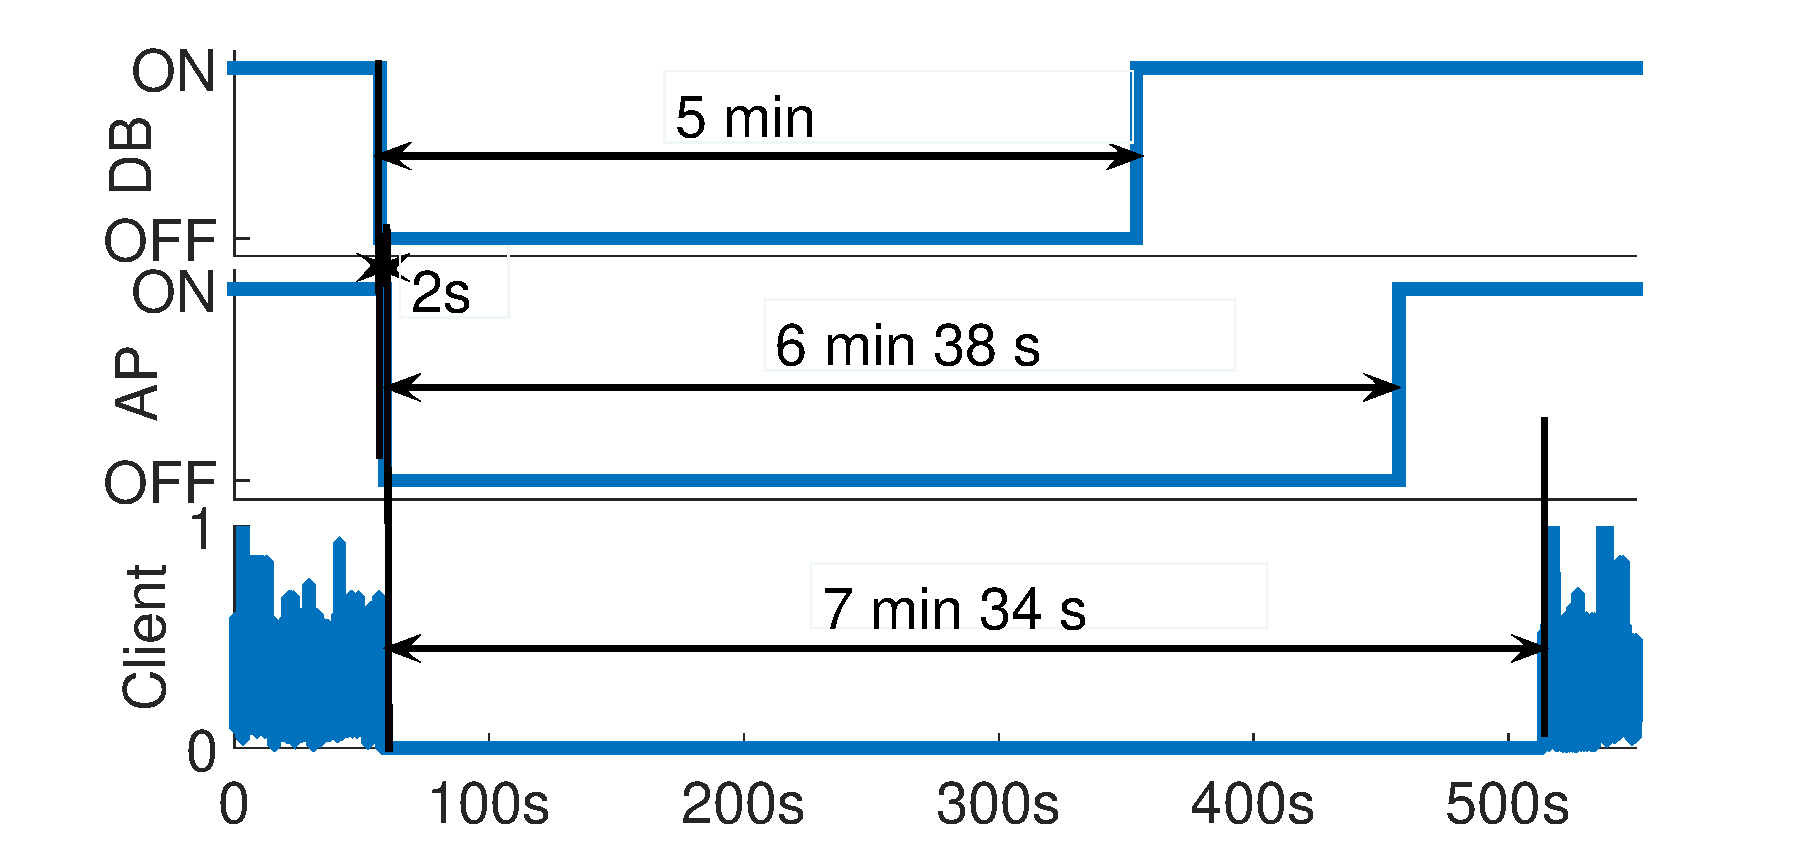
\includegraphics[width=0.5\textwidth]{./figs/paws.pdf}
  \vskip -6pt
  \caption{Spectrum database interaction experiment: At 57sec channel is removed from the database for 5 min, 2sec after later the AP radio is off and the client stops transmitting.}
  \label{fig:paws}
  \vskip -6pt
\end{figure}

%We see that 2sec after the channel has been removed, the radio is off. The client stops transmitting at the same time. This is well below the 60sec ETSI \cite{etsi_tvws} requirement. 

AP takes 1min 36sec to start the radio after channel is reintroduced. This is because our interface with the AP requires an AP reboot after any radio parameter changes so once the channel is reintroduced. We note that this process can be shortened using more advanced AP control interfaces such as TR-069~\cite{tr69}. 

Once the AP is on, it takes another 56s for a client to connect and resume traffic because it has to perform cell search on various frequencies in multiple LTE bands. This time can be further reduced by disabling unused LTE bands, which we are unable to do on our existing clients. 

\begin{figure*}[htb!]
  \hfill
  \begin{minipage}{0.15\textwidth}
    \centering
    (a)
    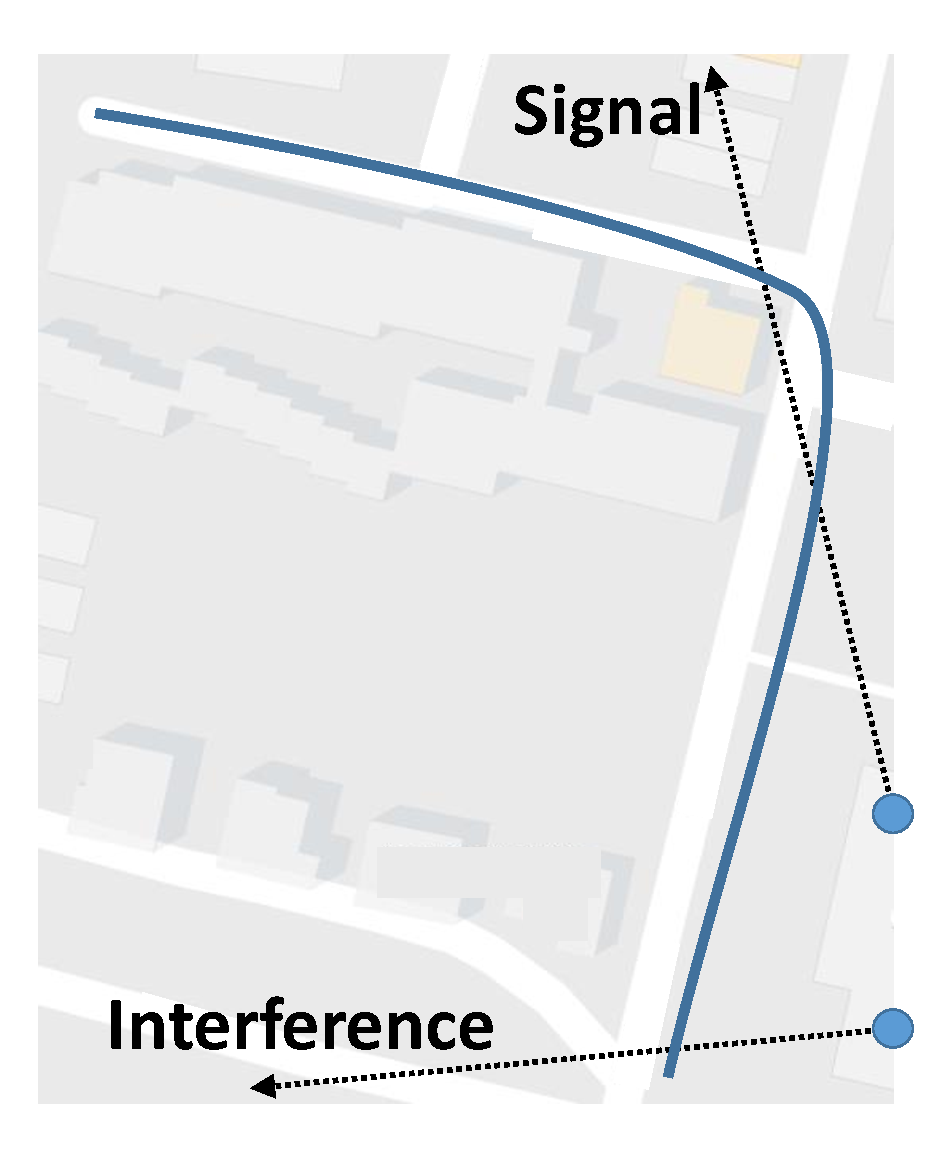
\includegraphics[width=\textwidth]{./figs/outdoor.pdf}
  \end{minipage}
  \hspace{12pt}
  \begin{minipage}{0.4\textwidth}
    \centering
    (b)
    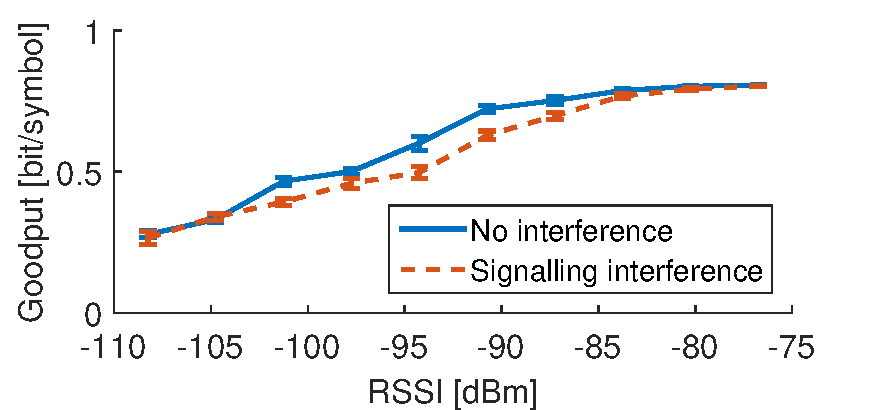
\includegraphics[width=\textwidth]{./figs/sig_vs_no.pdf}
  \end{minipage}
  \begin{minipage}{0.4\textwidth}
    \centering
    (c)
    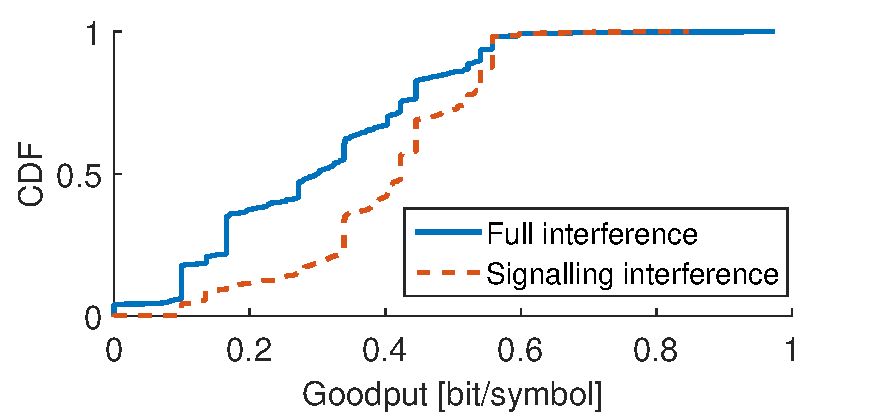
\includegraphics[width=\textwidth]{./figs/sig_vs_int.pdf}
  \end{minipage}
  \hfill
  \caption{Outdoor LTE interference experiment setup (a), 
  the difference between no interference and signalling-only interference (b) 
  and the difference between signalling-only interference and data interference (c).}
  \label{fig:interf_control}
\vskip -6pt
\end{figure*}



\subsection{Interference management}
\label{sec:interfeval}

As discussed in Section~\ref{sec:implementation}, we are unable to implement the interference management component due to software limitations of our small cell. Instead, we evaluate its key building blocks in a test-bed, and its network-level performance in large-scale simulations.



%% Second, we examine the effect of signaling and control channel interference on our design. 
%% Third, we examine whether CQI reports provide an accurate indicator of channel quality. 
%% Finally, we implement a PRACH detector using our software-defined radio to evaluate its complexity.


%\subsubsection{Signaling and control channel interference}
\subsubsection{Interference management with subchannels}

Interfering cells can mitigate inter-cell interference by avoiding to use the same subchannels at the same time.
This is not immediately obvious as LTE control elements are always present and can create interference 
even when there is no data being transmitted. This is particularly pertinent when a client is closer to an interfering cell than its serving cell. 

To understand the impact of control channel interference, we perform outdoor experiments with two E40 small cells, one acting as a serving cell and the other as an interfering one. 
The deployment is depicted in Figure~\ref{fig:interf_control}(a). 
Both cells are placed on the rooftop of our building, 15m high. The dashed lines depict the direction of each of the two antennas, and the solid blue line depicts the path over which we walked with a mobile device and performed the measurements. The end of the path is at about 250m from our building. We note that we have walked even further but due to the topology of the area the signal remains stronger than the interference and the results were similar to the ones at the end of the current path. We observe a large variability in SINR values, from -15dB to +30dB. We get such low SINR values because one end of the path is in the direction of the interference and outside of the main direction of the serving cell antenna.

We measure performance using Qualcomm's QXDM tool at the client and we log the received signal levels (RSSI) from one or both cells and the client's goodput in bits per symbol, where 
$ \mbox{bit}/\mbox{symbol} = \mbox{coding rate} \times (1-\mbox{BLER})$. 
We express goodput in bits per symbol rather than application-level throughput because our cell serves other users as well; hence, we measure throughput only within the resource blocks allocated to the test client.

We perform three measurements on the client's performance on the path: i) when only the serving cell is active, ii) when the interfering cell is active but has no users and iii) with the interfering cell being 
fully backlogged downstream. 
%first measure the client's performance on the path when only the serving cell is active. 
%In the second experiment we measure the client's performance on the same path when the interfering cell is active but has no users, hence it only emits control signals, creating control channel interference. In the third experiment we attach a user to the interfering cell and create a fully backlogged downlink. 
Figure~\ref{fig:interf_control}(b) shows the goodput as a function of the received signal strength for the case of no interference and signalling interference. The two vary by at most 20\% and in most cases much less than that. 
Hence, the control channel interference on its own does not affect the performance of data transmission significantly, even with SINR as low as -15dB. 
Figure~\ref{fig:interf_control}(c) presents the CDFs of the achieved goodputs with control channel interference only and with full data interference. 
We consider only the points where SINR is below 10dB, as in the other cases the goodput does not get affected much. We see that data interference can reduce the throughput by as much as 50\% in some cases. 
Also, we observe frequent disconnects at one end of the path when data interference is present, which we don't observe with control channel interference 
(disconnections are not included in the figure as we cannot register goodput during these intervals). 

Overall, data interference is critical in an LTE system.
Yet, two cells can share the spectrum successfully if they can coordinate data access in a way that we propose in Section~\ref{sec:archint}, despite interference from the control plane. 
We use these measurement results in our simulations to account for the effects of control-channel interference. 




\subsubsection{CQI \& channel quality}
\label{sec:eval_cqi}

The distributed subchannel selection algorithm is based on detecting subchannel interference from CQI reports (Section~\ref{sec:sensing}). 
We now demonstrate that CQI is a sufficiently accurate estimator of interference. 

Our CQI estimator needs to balance two challenges. First, channel quality fluctuates due to changes in the environment.
Second, an interfering signal might be weakened due to fading and not affect the overall throughput. 
The estimator should not trigger subchannel reallocation due to mis-identification of interference or when 
the interference signal is weak as this could result in loss of throughput; this will not allow the network to converge. 
These effects are highlighted through real measurements in Figure~\ref{fig:interf_control_time}. 
Due to fluctuating channel conditions, throughput varies significantly in the second OFF period, even when no interference is present.
Further, the last ON period shows the effect of fading, where despite interference being present, its signal is weak thus not affecting the overall throughput.

While \cf requires subband CQI reporting, our commercial small-cell access point does not implement the full LTE spec 
and only reports wide-band CQI over the entire 5 MHz channel. Thus, we only use wideband CQI reporting for this experiment. 
Yet, the same observations apply.

Our estimator works as follows. Since interference is typically bursty, we consider the maximum CQI observed within a time window as an estimate of CQI for a channel without interference. 
We declare that interference is present if we observe a CQI report below 60\% of this maximum value over a window of 10 consecutive samples. 
We measure the false positives by running the detector over samples of the channel without interference. 
We observe that it has less than 2\% false positives, i.e., one false positive every 100ms on average
(CQI is sampled every 2 ms). 
Our measurements further show that when interference is strong, our detector correctly reports interference with 80\% probability.
As with the interference measurements, we use these results in our simulations to model imperfect interference detection. 

%% Figure~\ref{fig:cqi} presents the accuracy of the estimator when interference is present, as a function of the level of interference.
%% The figure shows that when interference is strong, our detector correctly reports interference with 80\% probability.

\begin{figure}[t]
  \centering
    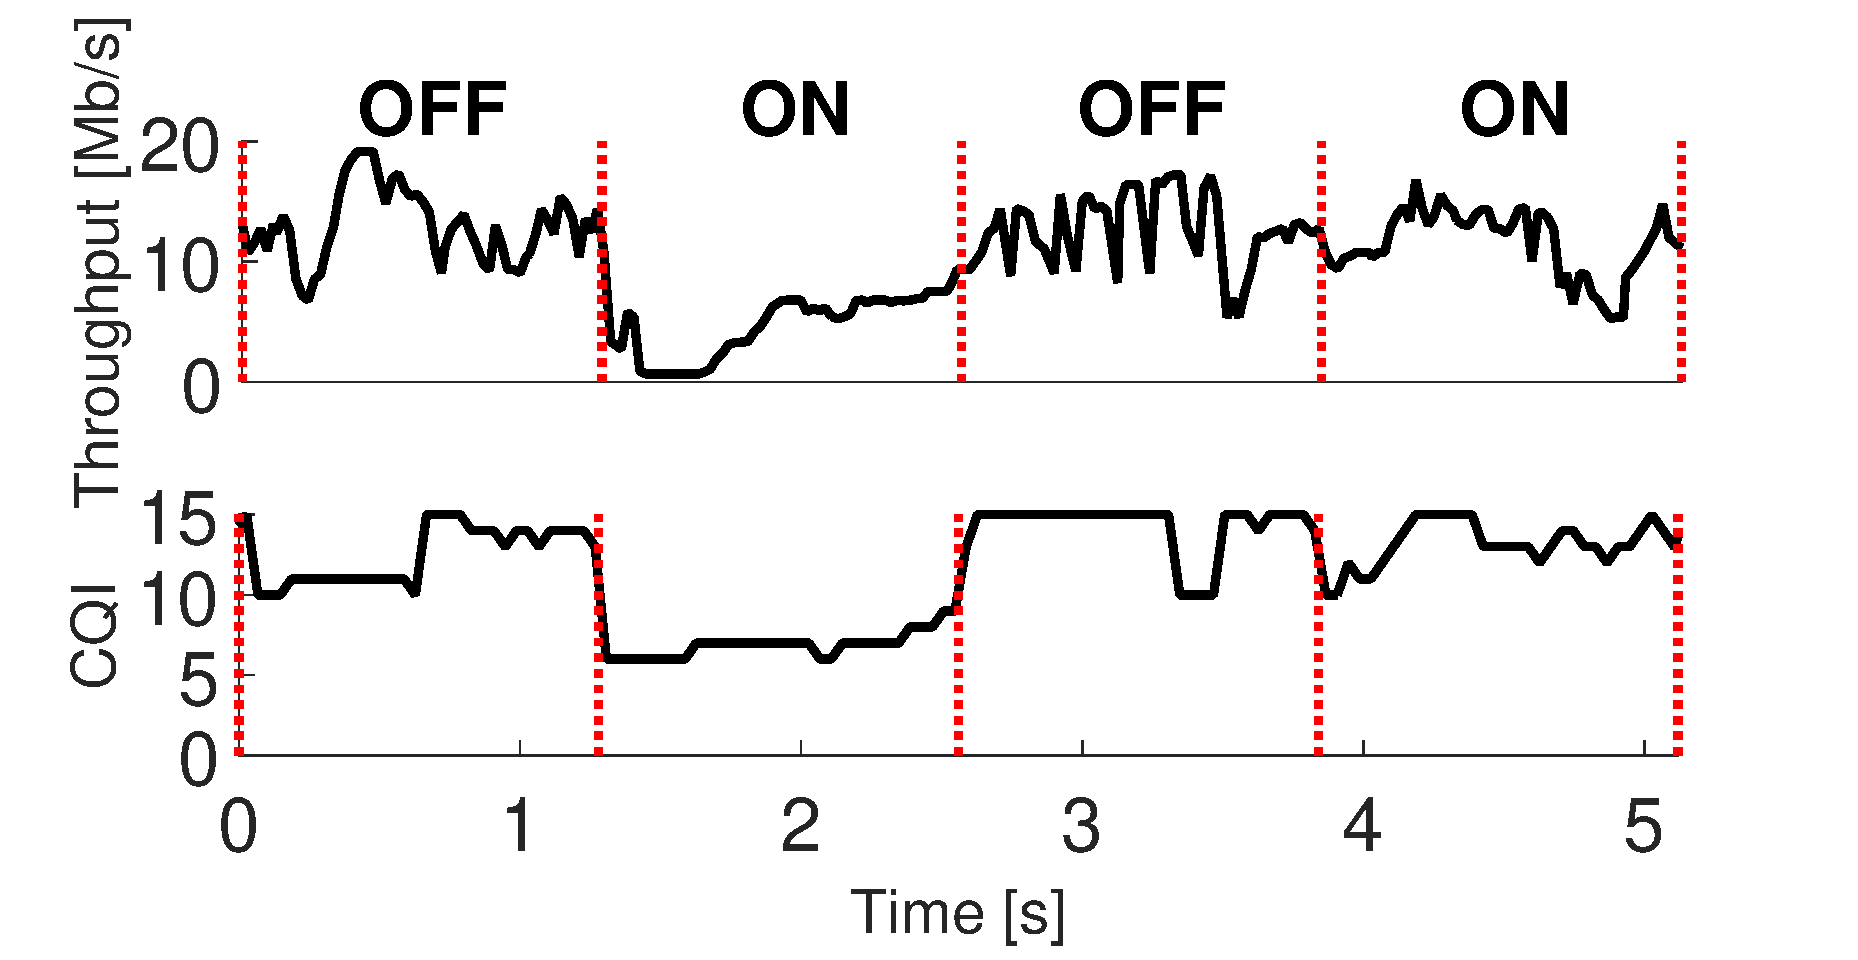
\includegraphics[width=0.5\textwidth]{./figs/cqi_time.pdf}
    \vspace{-0.3in}
  \caption{PHY throughput and channel quality indicator (CQI) reported during four states of interfering radio. 
ON denotes times where there is interference. }
  \label{fig:interf_control_time}
\vskip -6pt
\end{figure}

%% \begin{figure}[t]
%%   \centering
%%     \includegraphics[width=0.5\textwidth, height=0.4\columnwidth]{./figs/CQI.pdf}
%%     \vspace{-0.3in}
%%   \caption{Channel quality indicator (CQI) detection vs. the relative rate of interference.}
%%   \label{fig:cqi}
%% \end{figure}




\subsubsection{PRACH preamble detection}
\label{sec:pracheval}

\cf uses PRACH to estimate the number of contending clients. 
It is known that PRACH preambles can be detected at -10dB~\cite{prach}.
Here, we show that we can design a low-complexity PRACH detector for that purpose.


%% Clients initiate connections by sending PRACH preambles to access points they are associated with at predefined time instants. 
%% The main parameter of a PRACH signal is a preamble sequence number. 
%% The PRACH waveform is created from a root sequence using a cyclic shift that 
%% corresponds to the preamble sequence number. 
%% The sequence number is chosen randomly by clients for each PRACH transmission, 
%% and is used by access points to resolve potential contention among multiple clients~\cite{LTEbullets}. 

The key challenge for an access point trying to overhear PRACH preambles from clients not associated with it, 
is detecting these preambles efficiently without knowing the preamble sequence number~\cite{LTEbullets} or having the timing information. 
A naive implementation would correlate several long PRACH sequences, one for each preamble sequence number, 
whenever new samples are received. 

We propose a different detector which leverages the structure of the preambles. 
If we correlate a PRACH preamble received with a time offset, it will have a cyclic shift in its frequency representation. 
Equally, a different cyclic shift will be caused by a different preamble sequence number. 
We only need to detect whether a preamble is present, and neither need to know which preamble sequence has been transmitted 
nor when the transmission has started. 
Thus, we only need to perform two correlations; one to detect the most likely cyclic shift and 
another to check its correlation value. 

We implemented the modified detector on the SDR platform.
The detector has a comparable performance to a conventional implementation (with timing information) 
when receiving PRACH signals from a commercial dongle. 
Overall, it is 16 times faster than the required line rate (when ran on an Intel i7 CPU on a 10MHz channel).








%!TEX root = main.tex

\subsubsection{Large-scale Evaluation}
\label{sec:eval}

We evaluate the performance and properties of \cf 's interference management in large scale networks using the ns3 simulator ~\cite{ns3url}. 
Simulations are parametrized based on the experiments in the previous section, (the control channel interference and imperfect CQI reporting).
Overall, the evaluation examines a set of static and dynamic traffic scenarios along three dimensions.\\[2pt]
\noindent $\bullet$ \emph{MAC effects on throughput and coverage} in presence of interference, and comparison against LTE and \wf. \\[2pt]
\noindent $\bullet$ \emph{Application-level performance} by measuring the page download times of a web-like workload. \\[2pt]
\noindent $\bullet$ \emph{Distributed subchannel selection}. We evaluate \cf's resource allocation 
against a centralized, oracle-based state-of-the-art OFDMA resource isolation scheme~\cite{fermi}.\\


\begin{figure*}[htb!]
  %\hfill
  \begin{minipage}{0.33\textwidth}
    \centering
    (a)
    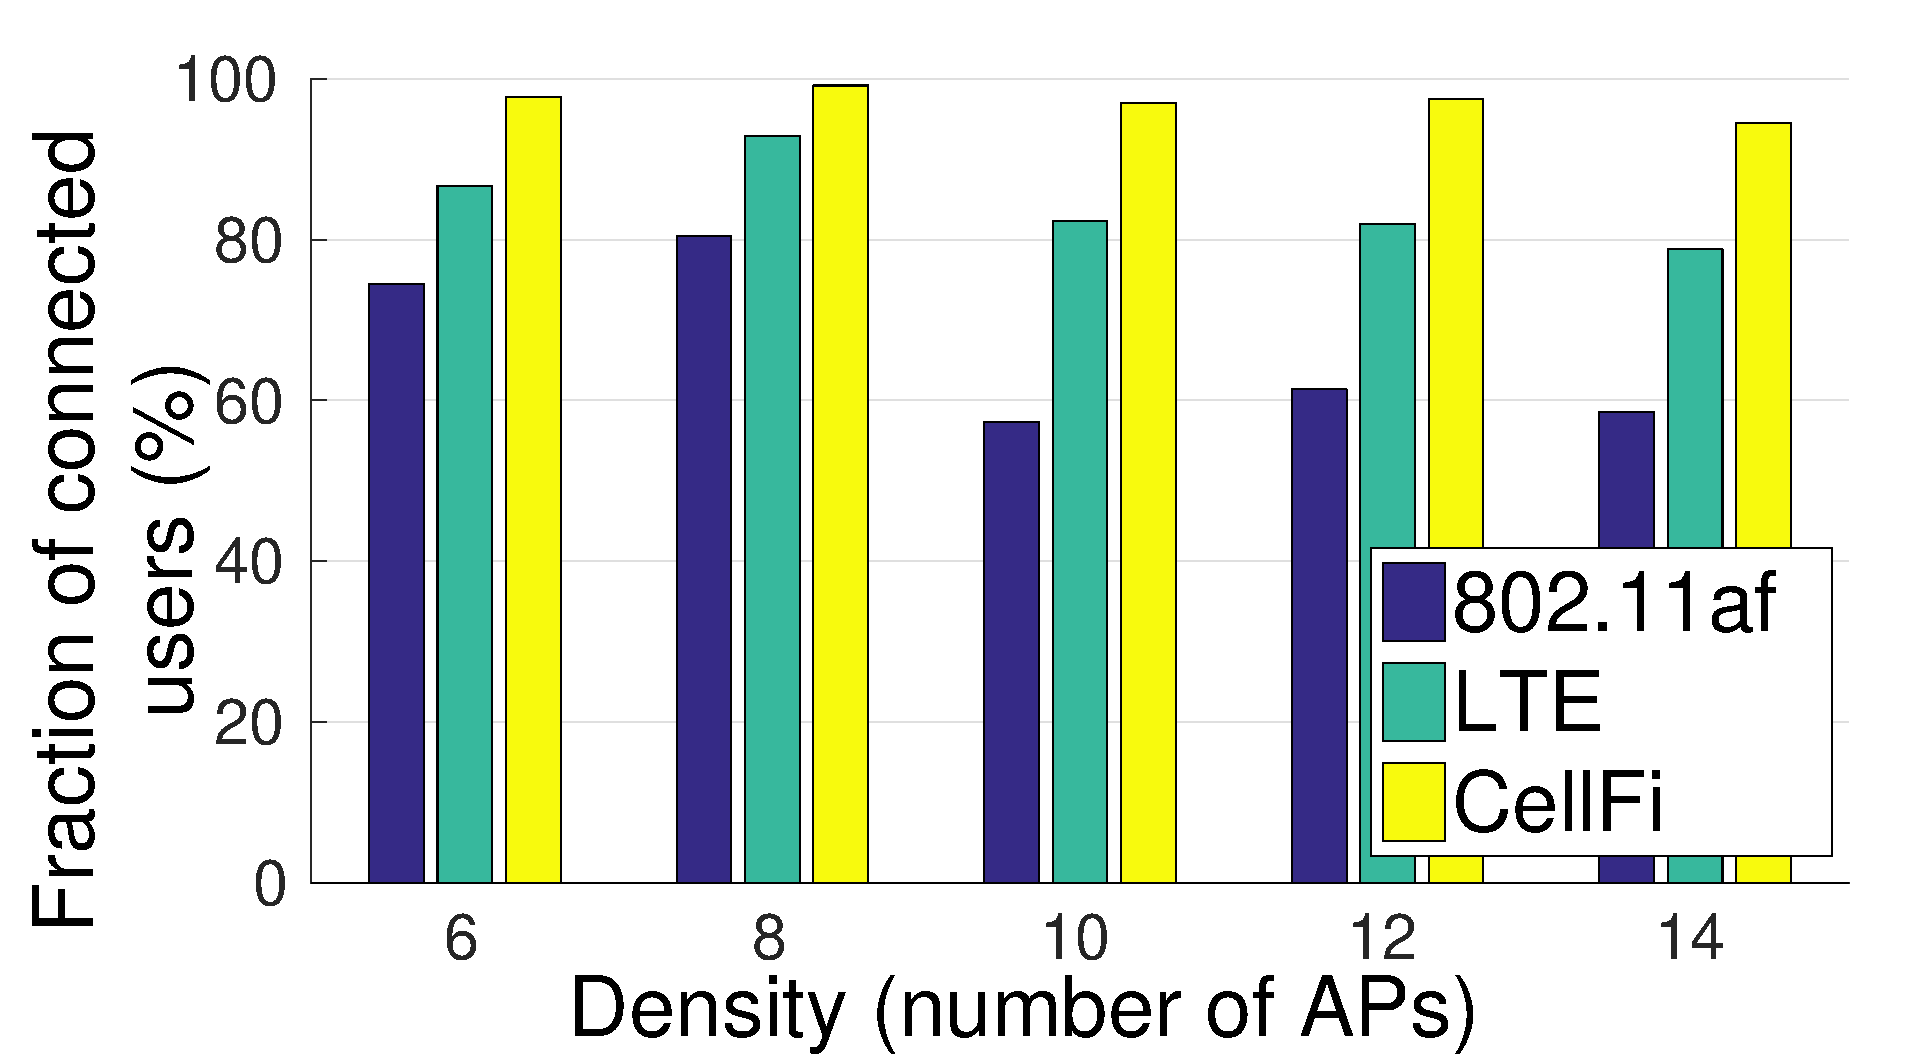
\includegraphics[width=\textwidth]{./figs/density-crop}
  \end{minipage}
  \hspace{1pt}
  \begin{minipage}{0.33\textwidth}
    \centering
    (b)
    \vfill
    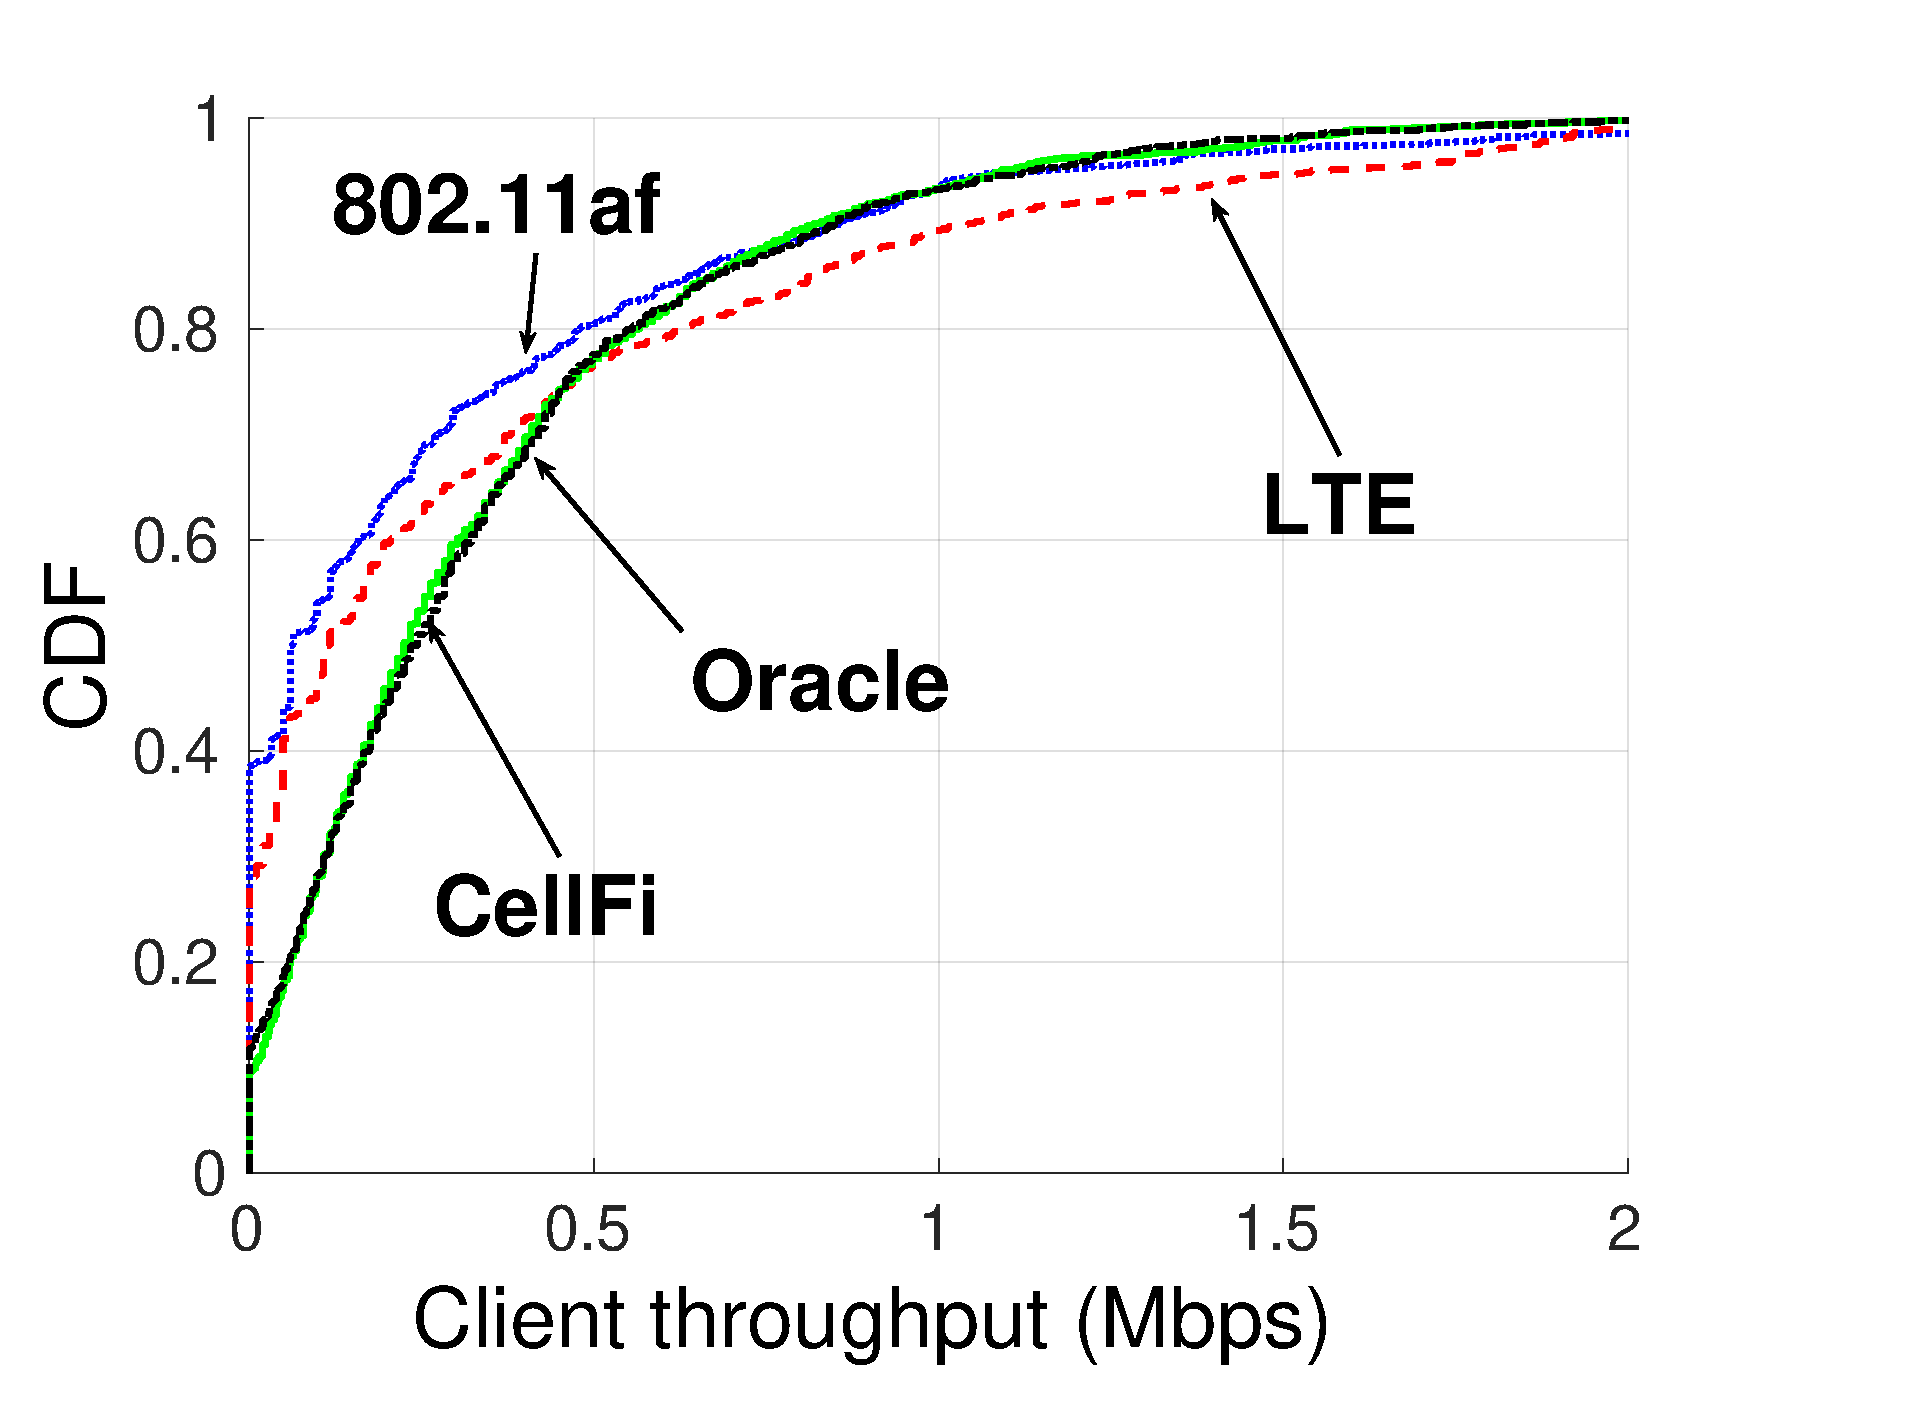
\includegraphics[width=\textwidth, height=0.55\columnwidth]{./figs/cli-crop}
  \end{minipage}
  \begin{minipage}{0.33\textwidth}
    \centering
    (c)
    \vfill
  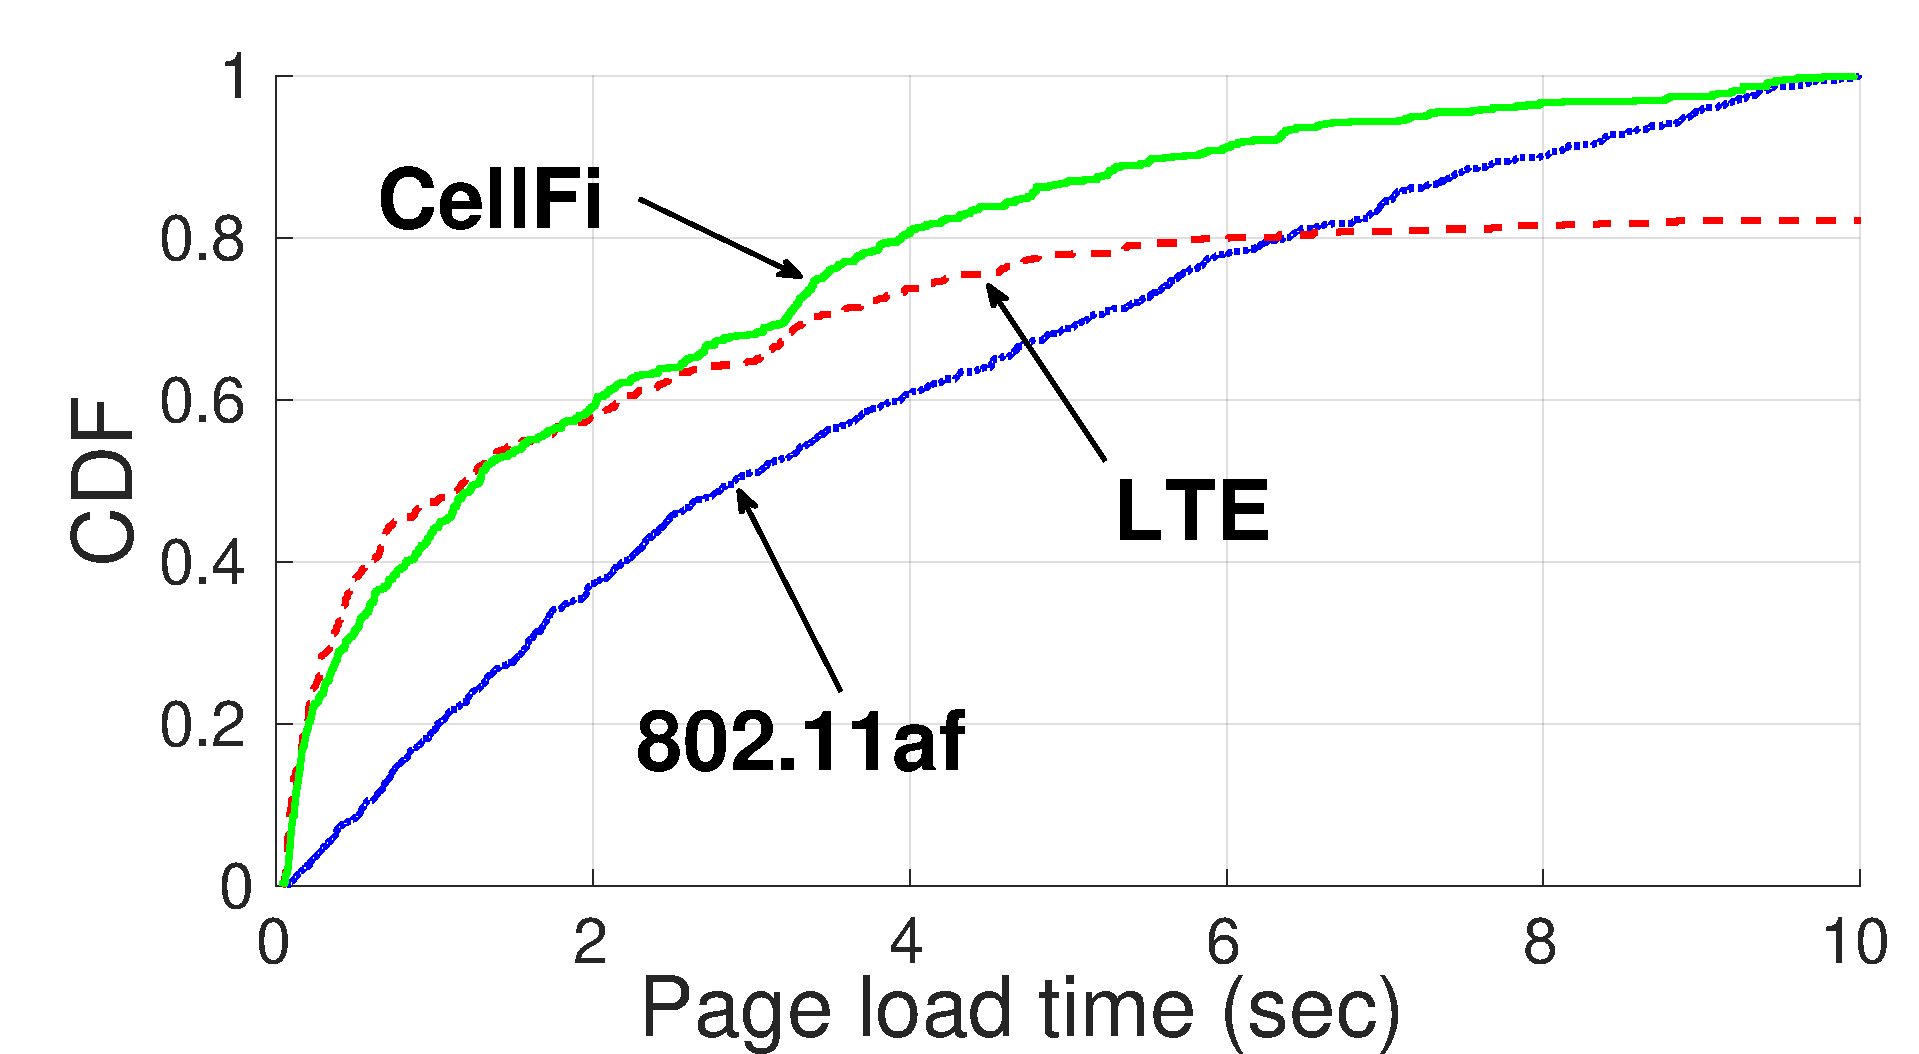
\includegraphics[width=\textwidth]{./figs/FCT-crop}
  \end{minipage}
  \hfill
\vskip -6pt
  \caption{Coverage vs density for \cf, \wf and LTE for 6 clients (a), 
    client throughput of \cf, \wf, LTE and the oracle (b), 
    page load times of \cf, LTE and \wf (c).}
  \label{fig:simulations}
%\vskip -6pt
\end{figure*}



\noindent{\bf Simulation settings.} 
%\label{sec:simset}
We simulate an area of 2 km x 2km, with a varying network density as controlled by the number of simulated APs. 
Base stations are randomly placed in this area with varying number of clients per AP. 
Unless otherwise noted, every scenario is repeated 20 times on a new topology. 

{\em Workloads.} We consider two types of traffic workloads and focus on downlink traffic. 
First, backlogged flows for all clients are used for throughput measurements. Second, 
we model web-like traffic based on realistic parameters regarding flow size, 
number of objects per page~\cite{trafficmodel} and thinking time distributions~\cite{thinktime}. 


%\begin{itemize}
%\item 802.11 VHT mac rates used, mcs 0 - 8 supported
%\item Ideal rate adaptation 
%\item maximum aggregation threshold used (65KB)
%\item RTS/CTS enabled, very low overhead due to high aggregation (without RTS/CTS results are worse)
%\end{itemize}

{\em \wf parameters.} We simulate 802.11af by adjusting the standard 802.11ac PHY and MAC layer in ns3 to match the 802.11af specs~\cite{Rice_af}. 
%with supported VHT MAC rates. 
Our \wf implementation uses ideal rate adaptation based on the 
receiver's SINR value, and supports MPDU aggregation with maximum possible aggregated frame size of 65 KB. 
RTS/CTS is enabled; its overhead is small due to the large aggregation and \wf performance is better with RTS/CTS.
The channel bandwidth for WiFi is set to be 6 MHz.

{\em LTE parameters.} We use the standard ns3 LTE implementation. For \cf, we added 
control channel interference and CQI detection probabilities, both derived from our measurements (Section~\ref{sec:interfeval}).
We choose 5MHz channel and TDD type 2, configuration 4~\cite{36_211} which grants 7 downlink (7ms) and 2 uplink (2ms) subframes in every 10ms frame.
%, which has similar efficiency compared to WiFi, as discussed in Section~\ref{sec:wifilimitations}. 


{\em RF.} WiFi and LTE support different PHY data rates, yielding different coverages. 
We choose the transmit powers for the two networks that provide the same coverage in isolation, 
in order to focus on MAC-layer efficiency.
For WiFi, TX power of both AP and client is set to be 30 dBm. For LTE, TX power of AP is 30 dBm and client is 20 dBm. 
We model loss propagation and noise floor based on our range measurements (Section~\ref{sec:PHY}).



\vskip 2pt
\noindent{\bf Coverage and throughput.}
We have already shown in Section~\ref{sec:PHY} that the link range can go beyond 1km when there is no interference. 
Here, we examine coverage when interfering cells are present. 
We use the static traffic workload and we compare \cf against \wf (802.11af) and LTE.
We also examine the performance a centralized oracle subchannel allocation~\cite{fermi} can achieve.
This provides the extent of performance loss compared to an optimal offline allocation.

Figure~\ref{fig:simulations}(a) shows how coverage varies as the network densifies. 
\cf improves coverage (number of connected users) 
and reduces the number of starved nodes compared to both \cf and LTE. 
For 6 clients per AP and 14 APs, coverage increases by 37\% and 16\% compared to \wf and LTE respectively. 
In an even denser scenario with 16 clients (not shown due to lack of space), 
\cf still offers coverage to more than 80\% of users, an increase of 32\% and 8\% compared to \wf and LTE. 

We now drill down in more detail and examine the performance offered in the densest of the scenarios with 6 clients of Figure~\ref{fig:simulations}(a).
This reflects 84 concurrent clients in a 5MHz channel; note that a typical 3G macro-cell today supports 32 active clients on the same bandwidth~\cite{quora}. 
Figure~\ref{fig:simulations}(b) presents the CDF of client throughput achieved across 20 runs of the experiment.
We observe that \cf improves the overall coverage and fairness, without sacrificing the total throughput in the network.
On the contrary, while with \wf and LTE some clients enjoy higher throughput, this is at the expense of 30-40\% of starved clients due to 
exposed and hidden terminals in the case of \wf, and lack of interference management in the case of LTE. 
Overall, \cf roughly doubles the total throughput achieved per AP compared to \wf at the median, while 
reducing starved clients by roughly 70\% compared to LTE and \wf. 
We also observe that \cf always provides connectivity to more than 90\% of the clients,
while there are cases were \wf and LTE only provide connectivity to 30\% and 60\% of clients respectively.
Note that \cf presents near optimal performance when compared to 
the oracle subchannel allocation (Figure~\ref{fig:simulations}(b)). 



\noindent{\bf Application-level performance.} 
To understand \cf's impact on real applications, we model dynamic traffic conditions based
on our web workload, and examine web-page download times. 
Figure~\ref{fig:simulations} (c) presents the corresponding CDFs of page completion time. The figure
highlights that \cf reduces completion times by 2.3 times at the median compared to \wf, 
and roughly by 8\% relative to LTE. LTE provides marginally better times at smaller percentiles, however
tail performance is significantly degraded due to interference. We also examined whether the network converges. 
We observe that the vast majority of access points only hop very few times in all of our runs; roughly 
1\%-2\% of access points do not converge due to interference and hop almost continuously. 
We omit these figures due to space limitations.

%In Figure~\ref{fig:fct} (right) we plot the CDF of number of channel hop per AP over all runs, normalized by the highest hop number. 
%We see that there is a small fraction of APs that always hop, which are a few starved nodes. 
%Most of the other nodes converge fairly quickly, which explains the observed performance benefits. 


%XXX add discussion about convergence.

%\begin{figure}[h!]
%  \centering
%    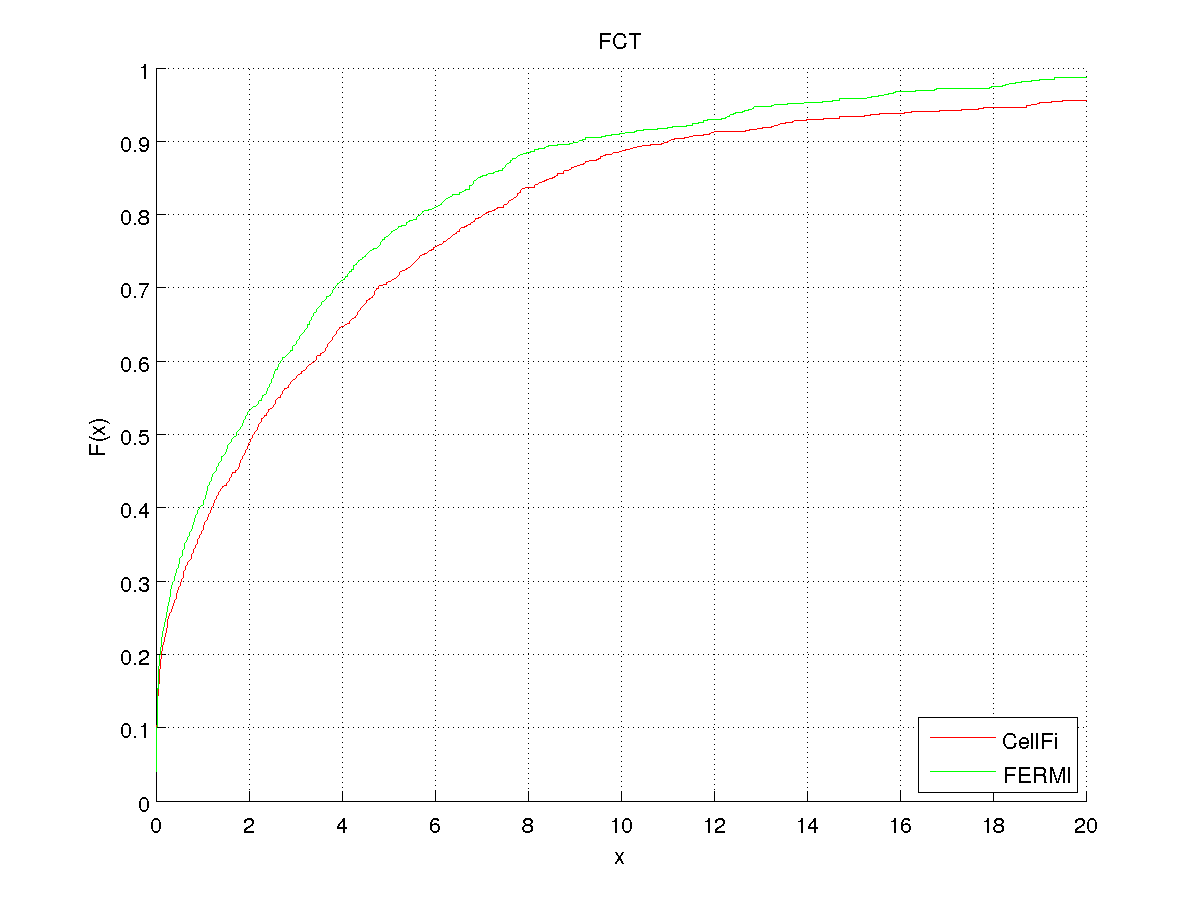
\includegraphics[width=0.5\textwidth]{./figs/FCT-fermi.png}
%  \caption{FCT comparison with FERMI}
%  \label{fct}
%\end{figure}



%\subsubsection{Rate allocations}

%In \ref{minFERMI} and \ref{totalFERMI} we compare CellFi with FERMI~\cite{fermi}. 

%\begin{figure}[t]
%  \centering
%    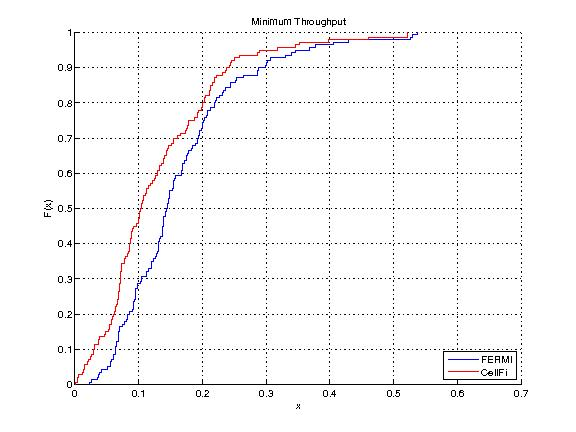
\includegraphics[width=0.45\columnwidth]{./figs/min_CellFi-FERMI.jpg}
%    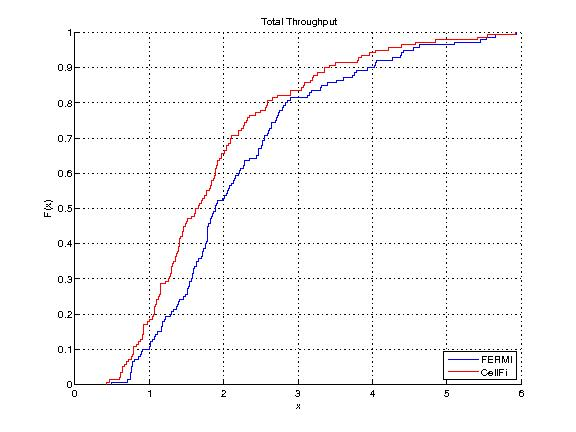
\includegraphics[width=0.45\columnwidth]{./figs/total_CellFi-FERMI.jpg}
%  \caption{Minimum (left) and total (right) throughput of \cf vs the oracle}
%  \label{minFERMI}
%\end{figure}

%\begin{figure}[h!]
%  \centering

%  \caption{Total Throughput Comparison with FERMI}
%  \label{totalFERMI}
%\end{figure}



\noindent{\bf Overheads of signaling.}
CellFi uses mode 3-0 higher layer configured sub-band CQI feedback reports, which consists of 1 wideband CQI value (4 bits) and 13 sub-band CQI values (2 bits). 
The payload size for a single mode 3-0 report on a 5 MHz channel is 20 bits per report. 
The overhead of signaling is 10 Kbps on the uplink for a reporting period of 2 ms. 

%(XXX comment on the overhead) 




%\section {Discussion}

In this section, we mention a number of important points related to \cf design that have not been discussed.

\noindent {\bf Coexistence between \cf and 802.11af:} \cf focuses on coexistence among LTE nodes. There are several other efforts (LTE-U, LAA, LWA) that look into coexistence between LTE and WiFi. 
These are orthogonal solutions that could be
deployed along \cf to enable coexistence with 802.11af. 

\noindent {\bf Centralized vs distributed control plane:} \cf deploys a decentralized control plane. We show that it is efficient and comparable with the state-of-art centralized control plane~\cite{fermi}. 
We also note that \cf can be extended to include centralized coordination among nodes from one provider, and distributed coordination across multiple providers, which could further improve performance. 

\noindent {\bf Mobility and roaming:} \cf inherits the benefits of the LTE architecture.
It provides seamless roaming across access points, which is difficult to engineer in current WiFi deployments. 

\noindent {\bf Channel aggregation and power optimization:} \cf currently only uses a single TV channel for its operations. One can think of a more flexible channel allocation that will allow channel aggregation and optimization for power. However, these raises other challenges, such as how to detect interference in partially overlapping channels~\cite{whitefi}, which we leave as future work.

\noindent {\bf Ease of deployability:} \cf works with unmodified LTE base-band chipsets. However, it does require changes on the access point side. We note that the majority of LTE small cells today are built in software, on programmable reference platforms from TI, Freescale, Broadcom and Qualcomm. Hence we speculate that \cf can be implemented entirely in software on top of these commodity platforms. 



\section{Discussion and Related Work}








TV white spaces have recently become available for license exempt use~\cite{fcc, etsi_tvws}. 
There are several currently proposed candidate technologies, such as 802.11af~\cite{Rice_af} and 802.22~\cite{wifi80222}, 
but 802.11af seems to be the only one under active development. 

LTE extensions have recently been proposed that seek to exploit unlicensed spectrum~\cite{qualcomm-lte-unlicensed,huawei-lte-unlicensed,ericsson-unlicensed}, but all these require an anchor, licensed spectrum for the LTE network.
The main proposed standards are LAA, LWA and LTE-U. 
Previous works ~\cite{co-existence, lteu-google} focus on WiFi and LTE coexistence in unlicensed spectrum, but coexistence between two LTE networks on the same spectrum has not been studied much.

There are also numerous proposed solutions for coordinating interfering LTE access points, such as SON, ICIC, eICIC~\cite{smallcellbook}, 
but these are vague on protocol details. 
FERMI~\cite{fermi} proposes a centralized resource management solution in OFDMA networks, however it assumes cooperation among operators which is not realistic in our setting.
%http://alumni.cs.ucr.edu/~marslan/hoc19-yoon.pdf (radion)
RADION~\cite{radion} is a distributed resource management system designed for femtocell networks and does not scale well to large deployments.

WiFi channel allocation has been extensively researched. 
%http://www.cs.umd.edu/~srin/PDF/2006/chan-mgmt-conf.pdf
%http://ieeexplore.ieee.org/stamp/stamp.jsp?tp=&arnumber=5337940
%http://research.microsoft.com/en-us/um/people/moscitho/Publications/ICNP_2008.pdf
There have been several studies ~\cite{client-deriven} ~\cite{load-aware} that address resource allocation using graph coloring for WiFi networks, but their aim is to get maximum number of orthogonal contiguous channels to each interfering AP. Our work aims at getting weighted max-min fair allocation for interfering clients by utilizing as many spectrum fragments (not necessarily contiguous) as possible.
\wf 802.11af can be made to use more than one channel~\cite{whitefi}, and  LTE can achieve this with 
carrier aggregation. We leave exploring these options for future work. 

Several papers proposed the idea to use LTE in TV white spaces~\cite{dyspan_lte12, radisys} but none has described an
 architecture or proposed an efficient distributed interference management system compatible with today's hardware. 



\section{Conclusions}
We have designed \cf, a long-range LTE-based network operating in TVWS. \cf interfaces with a TVWS spectrum database and uses a fully decentralized interference management algorithm that allows for uncoordinated and unplanned deployment but is compatible with the existing LTE network stack. We show the feasibility of \cf using experiments with off-the-shelf LTE equipment. Our extensive simulation results show that \cf improves MAC performance compared to \wf and LTE by reducing the number of starved clients by 70\%-90\%, without affecting the total throughput of the network or penalizing application performance.




\bibliography{ref}
\bibliographystyle{unsrt}


%\appendix

\section{Appendix}


\subsection{Algorithm Properties}
\label{sec:proof}

%\todo{Dan will fill this in.}
%The reason why this work is our high-level design and the distributed share calculation. The distributed share calculation makes sure that the starting allocation is feasible. This allows us to do packing based on free channels. If the initial share wasn't feasible, the algorithm would have issues converging (Dan has a proof for this). This is why the packing idea is fundamentally suitable for our approach.

We now analyze the properties of the assignment framework given in ~\ref{sec:channel-selection}. 
In particular, we will give a sufficient condition under which the basic hopping algorithm 
(without the channel re-use heuristic) is guaranteed to converge, 
and probabilistic convergence bounds in this case. 

More precisely, we abstract the given setting as an undirected graph $G = (V, E)$, where each vertex $v_i \in V$ corresponds to an \eNB $i$. 
Further, two vertices $v_i$ and $v_j$ are connected by an edge if $v_i$ may interfere with one of $v_j$'s clients, or vice-versa. 
Let $N(v_i)$ denote the graph neighborhood of node $v_i$. 
Vertices share a set of $M$ subchannels, and initially each vertex $v_i$ has integer demand $d_i \geq 0$, which corresponds to the sum of user shares computed by the algorithm. 
Our analysis makes the assumption that, in every neighborhood, there exists a constant factor difference between the sum of demands and the total number of  subchannels.

\begin{eqnarray*}
  \textnormal{There exists a constant } 1 / M < \gamma \leq 1, \textnormal{ such that: } \\ \textnormal{ for every node }  v_i, \sum_{\ell \in N(v_i)} d_\ell \leq (1 - \gamma) M.
\end{eqnarray*}

Further, our analysis models subchannel fading by admitting a probability $0 \leq p < 1$ that a subchannel sensed as \emph{free} (and therefore chosen by the hopping procedure) is in fact unusable by the node. 
This failure event is assumed to be independent of the nodes' random hopping choices, and across hopping rounds. 

We focus on \emph{convergence time}, i.e., the time required for the algorithm to reach a configuration in which each node has its subchannel demand fulfilled, and stops hopping. 
We prove the following. 

\begin{thm}
\label{thm:convergence}
	Under the above assumptions, the algorithm is guaranteed to converge with probability $1$. The algorithm will converge in $O( M \log n / ((1 - p) \cdot \gamma) )$ rounds, both in expectation and with high probability.   
\end{thm}
\begin{proof}
	Let us consider the process by which a node $v$ satisfies a unit of its demand. By assumption, the following hold: 1) the node $v$ will not hop on a subchannel currently occupied by another node $v'$ and 2) since a node $v_\ell$ may only occupy $d_\ell$ subchannels in a round, and $\sum_{\ell \in N(v)} d_\ell \leq (1 - \gamma) M$, there exist at least $\gamma M \geq 1$ subchannels which are available at every hopping attempt. Therefore, given a hopping attempt by $v$, there are two conditions under which it does not succeed in acquiring the channel: either another node makes the same choice, or the channel is faded. These events occur independently, and, by assumption, the probability that node $v$ satisfies one unit of demand in a hopping attempt is at least $(1 - p) \gamma$.  
	
	Since round choices and fading are assumed to be independent across rounds, the expected time for the fixed node to satisfy a unit of demand is $ 1 / (\gamma (1 - p))$. By a Chernoff bound, for any constant $k \geq 2$, there exists a constant $c \geq 1$ such that the probability that the node fails to satisfy a unit after $k \log n / (\gamma (1 - p) )$ consecutive hopping attempts is at most $1 / n^c$. 
	By a union bound on the number of nodes, the probability that there exists \emph{some} node which fails after $k \log n / (\gamma (1 - p ))$ consecutive hopping attempts, is at most $1 / n^{c - 1}$. 
	The claim then follows by noticing that a node's demand is of at most $M$ subchannels. 
\end{proof}


It is interesting to consider the effect of channel packing on convergence. 
Technically, a larger channel slack $\gamma$ may be needed if hopping and packing occur concurrently, as packing may increase collisions. 
However, the fact that packing occurs after the node stops hopping ensures that the two procedures are independent to some degree.
The empirical evaluation confirms that convergence still occurs with packing, even for dynamic traffic patterns. 




%If  $Share_{ij}$ was decreased from this phase is lesser than the previous phase the eNB picks new sub-channels equal to the difference based on the reported CQI from $client_j$, if its greater eNB picks the best sub-channels from the ones previously assigned to $client_i$ that satisfy the new share.

%% \subsubsection{Implementation Details}
%% \label{other}

%% \noindent We now specify some key  implementation details. 


%% \noindent {\bf Channel Packing:} 
%% A useful optimization is the efficient packing of clients to channels, to enable spatial reuse. 
%% For example, clients which are very close to their respective base-stations are not likely to interfere with each other, and hence it would be beneficial for them to get the same allocation. 
%% While this is difficult to achieve without additional coordination, our design uses the following heuristic: 
%% each client maintains a leaky bucket corresponding to each channel it is assigned to. 
%% The client will move to a channel \emph{of lower index} if this channel is detected as \emph{free} for a certain contiguous period of time. 
%% The idea is that clients which experience low interference (such as the ones close to the base-station), will gradually move towards lower-index channels, and spontaneously self-organise. Moreover, as observed on the test topologies, convergence is reasonably fast. 




%% \noindent {\bf Scheduling:} Resources are allocated to an access point using the algorithm above. However, they are not strictly assigned to any specific client. Each access point can schedule any of its clients into any of the resource blocks it has acquired using any local scheduling algorithm. In our evaluation, we use the standard proportionally fair scheduling algorithm to schedule clients in order to achieve fairness across clients and combat channel selectivity. 

%% \noindent {\bf Detecting remaining interference: } As discussed in Section~\ref{issues}, an access point may incorrectly compute its share and take too many resources, due to sensing asymmetry. 
%% More precisely, the \eNB may believe that some resources are available, even though other access point potentially interferes on these resource blocks at the corresponding client. This type of interference is detected through client's CQI reports. If an \eNB observes a significant drop in the CQI for one or more resource blocks, the access point decides that the corresponding resource blocks are busy and removes them from the allocation.

%% \noindent {\bf Fairness in Cell-Fi:} There are several ways to define fairness in our context. We use temporal fairness for two reasons. The first is that it gives each user a the same time to access the spectrum, i.e. the shared resource. 
%% The second reason is that we can easily estimate the number of users, but not much else. Hence, any kind of proportional fairness based on rates is impossible, since we do not have any estimate of the rate. 

%% \todo{DAN: I think this discussion should be moved after the evaluation.} 
%% In our evaluation, we note that Cell-Fi tends to allocate more resources to remote nodes, when compared to other schedulers such as Fermi~\cite{fermi}. This reflects our choices of using low frequencies and focusing on coverage. 
%% Nodes which are closer to the \eNB can use higher frequencies to achieve connectivity. 


\begin{figure}[htb!]
  %\hfill
  %\begin{minipage}{0.33\textwidth}
  %  \centering
  %  (a)
  %  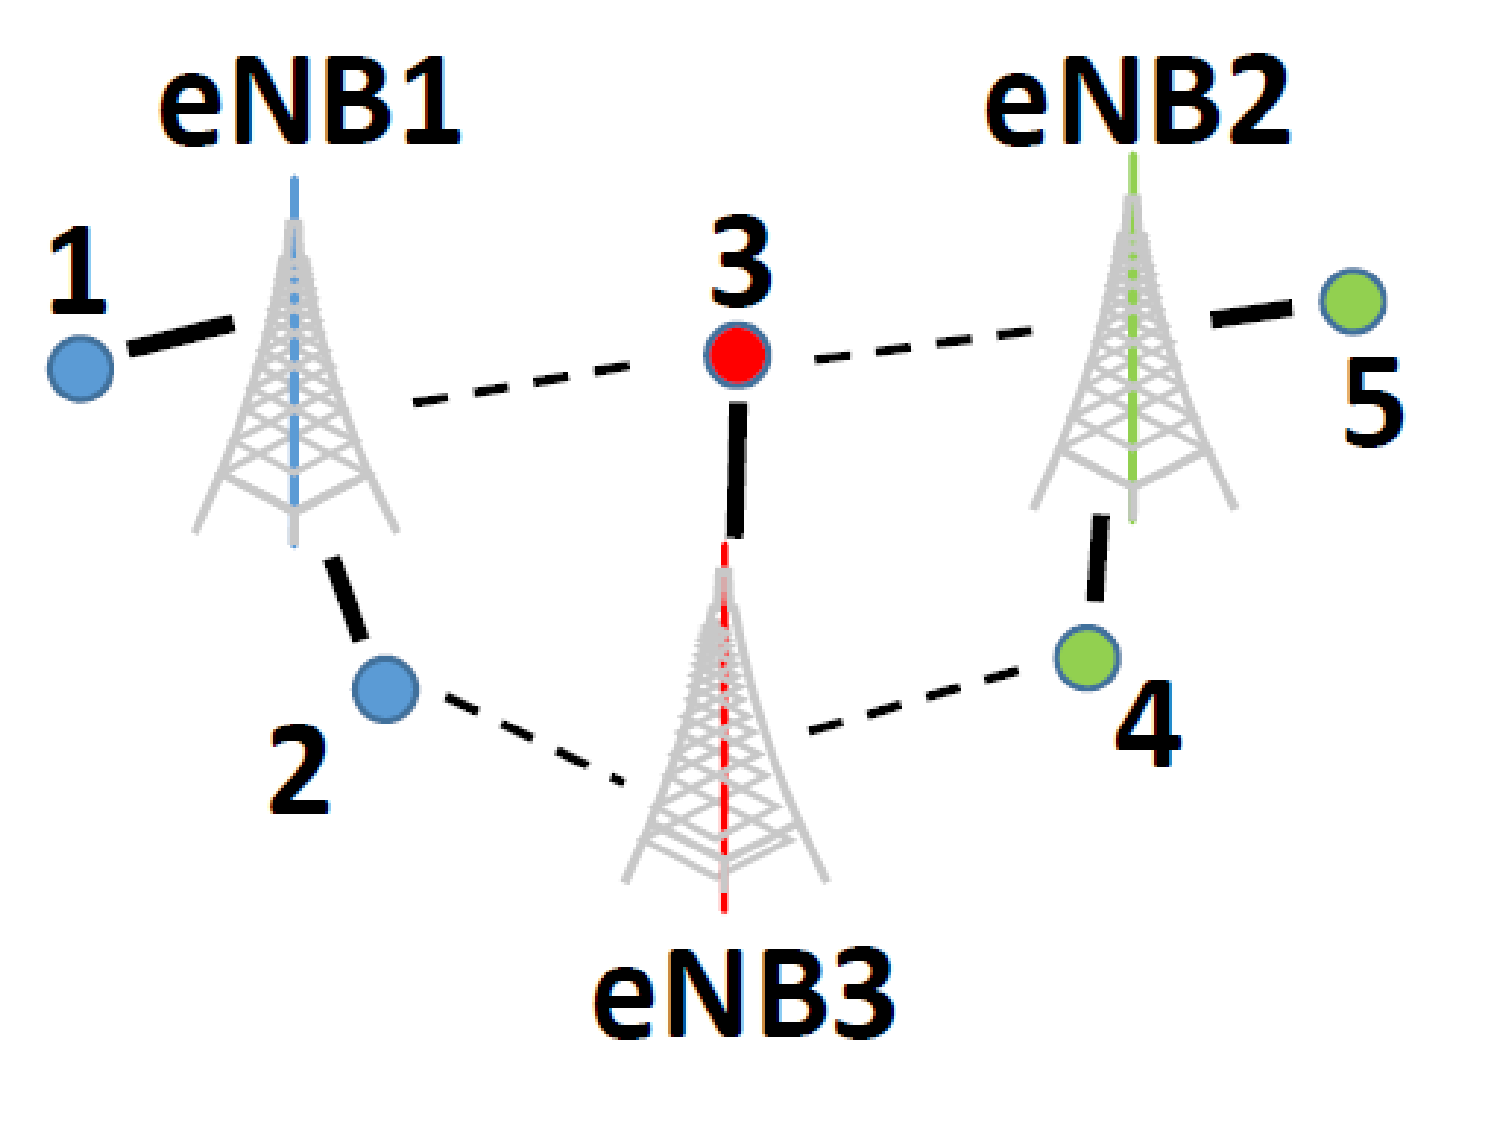
\includegraphics[width=\textwidth,height=0.6\columnwidth]{./figs/pack.pdf}
  %\end{minipage}
  %\hspace{1pt}
  \begin{minipage}{0.23\textwidth}
    \centering
    (a)
    \vfill
    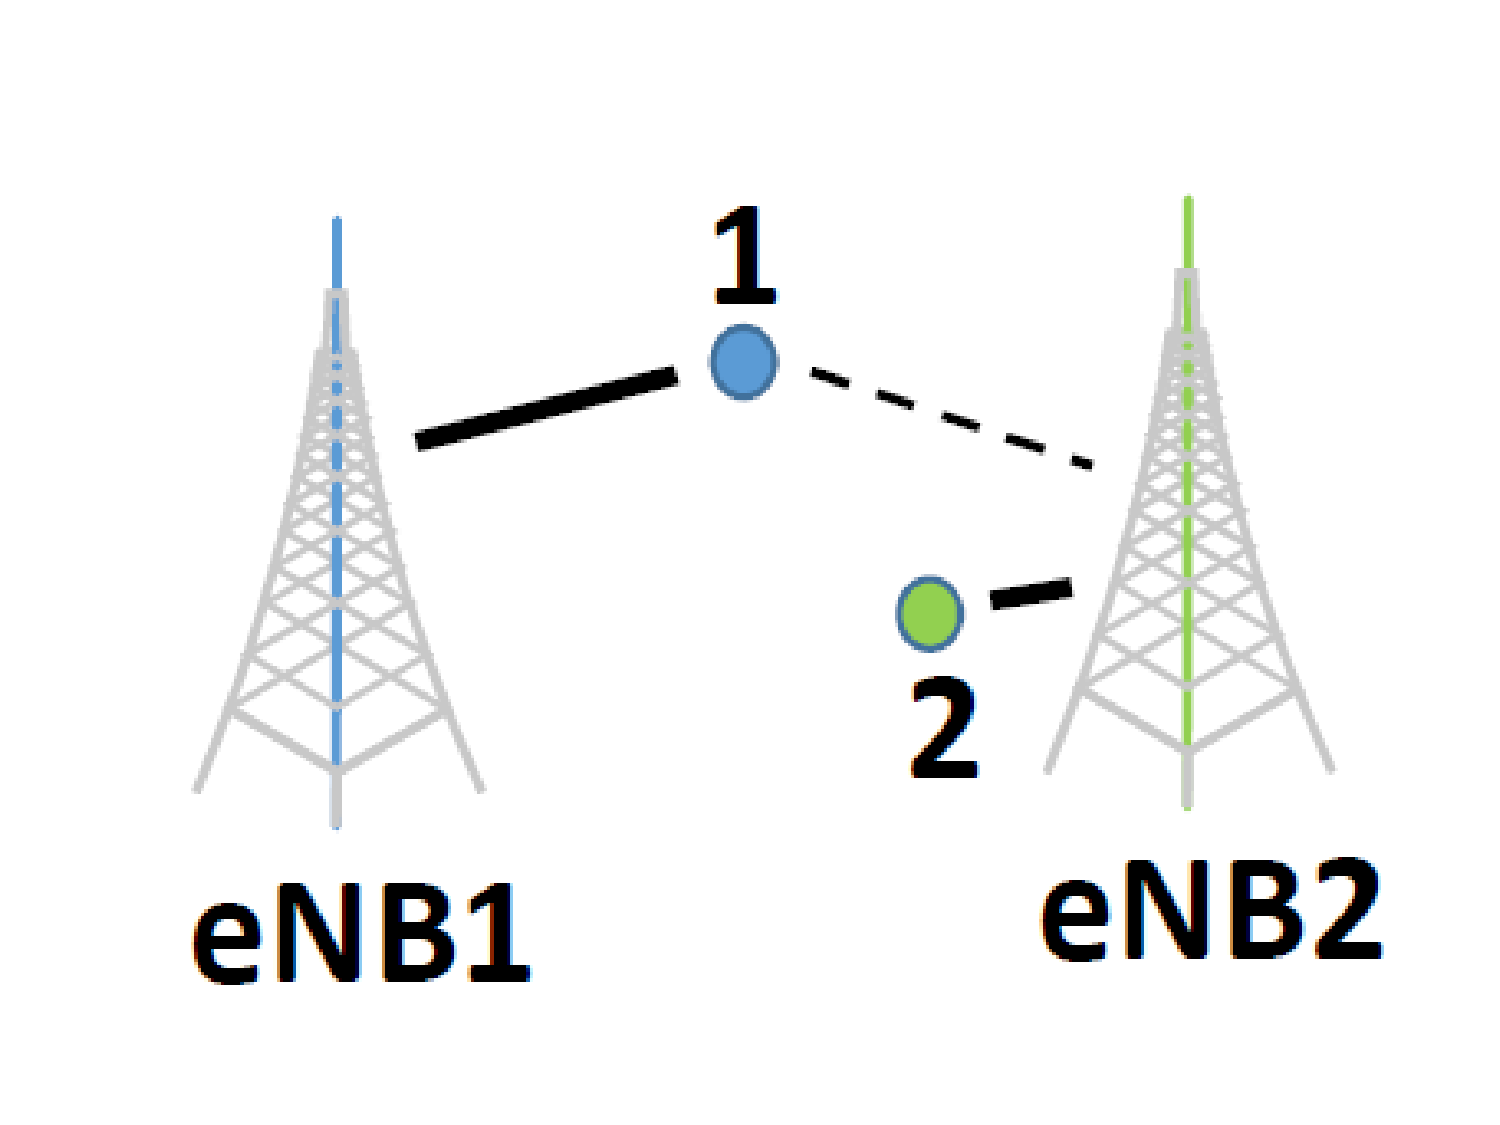
\includegraphics[width=\textwidth,height=0.6\columnwidth]{./figs/over.pdf}
  \end{minipage}
  \begin{minipage}{0.23\textwidth}
    \centering
    (b)
    \vfill
  \includegraphics[width=\textwidth,height=0.6\columnwidth]{./figs/under.pdf}
  \end{minipage}
  \hfill
  \caption{Lines reflect associated clients to access points while dashed lines reflect interference. }
%(a) Importance of channel re-use. client 3 can only get its share if access points 1-2 schedule their clients on same two channels. 
%(a) Information asymmetry with two total channels. access point 1 overestimates his share because it cannot sense client 2. (b) Informatrion assymetry with 4 total channels. 
%access point 2 has a share of 1, and while access point 1 can increase his share to 3, 
%it only reserves his fair-share, i.e., 2 channels because it does know how many subchannels 2 is using (1 due to clients 3-5)}
  \label{fig:asym}
\end{figure}


\subsection{Effects of information asymmetry}
\label{sec:asymmetry}


Wireless sensing depends on node location, and different nodes will obtain different views of the network. 
Every distributed wireless coordination protocol has to deal with this information asymmetry. 
The best known examples of information asymmetries in WiFi are exposed and hidden terminals. 
The distributed share calculation algorithm of \cf also suffers from two cases of information asymmetry, 
described below. 





%\begin{figure*}[t]
% \centering
%    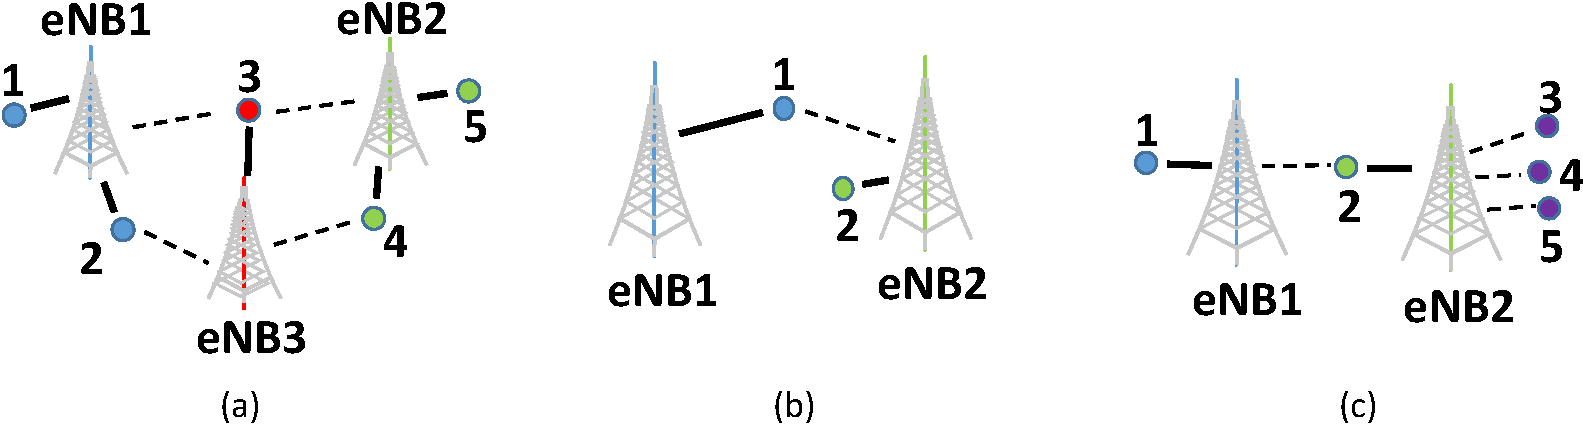
\includegraphics[width=0.9\textwidth, height=0.4\columnwidth]{figs/exampleFigs-crop}
% \caption{Lines reflect associated clients to access points while dashed lines reflect interference. 
%(a) Importance of channel re-use. client 3 can only get its share if access points 1-2 schedule their clients on same two channels. 
%(b) Information asymmetry with two total channels. access point 1 overestimates his share because it cannot sense client 2. (c) Informatrion assymetry with 4 total channels. 
%access point 2 has a share of 1, and while access point 1 can increase his share to 3, 
%it only reserves his fair-share, i.e., 2 channels because it does know how many subchannels 2 is using (1 due to clients 3-5)}
%  \label{fig:asym}
%\end{figure*}




\noindent {\bf Incorrect share:} Figure~\ref{fig:asym}(a) shows an example of incorrect share calculation caused by asymmetric views. 
access point 1 can hear only the PRACH preamble from client 1, whereas eNB2 hears it from both clients 1 and 2. The optimal share for both eNBs is half of the spectrum. 
Because of asymmetry, access point 1 is overestimating its share to be the whole spectrum.

%BR: This is not true. If we don't adjust the share, it will make eNB1 to hop a lot, causing disturbances in the rest of the network...
%This case of information asymmetry is not detrimental to the control plane. It does not affect client 2 because if it did eNB1 would hear it RACH and account for it in the channel allocation. It only affect client1. eNB1 detects this from CQI reports from client1 and adjusts the allocation accordingly and entirely locally. 

This case of information asymmetry is dealt with by the scheduler, \eNB $1$ will sense that there are less free subchannels available than it expected, and will not schedule any transmission in subchannels the client is facing interference on, reducing its effective share. The resulting effective share will still be feasible, allowing the distributed hopping algorithm to converge. However, this share adjustment may not be detected by other neighbors of \eNB $1$, leading to possible inefficiencies.
%in the share calculation algorithm (Figure~\ref{fig:dsc}) 
%through the $\id{free}_{i, j}$ variable. \eNB $1$ will sense that there are less free channels available than it expected, and will update its share. The resulting share will still be feasible, allowing the distributed hopping algorithm to converge. However, this share adjustment may not be detected by other neighbors of \eNB $1$, leading to possible inefficiencies. 

%\begin{figure}[th!]
%  \centering
%    \includegraphics[width=0.45\textwidth]{under}
% \caption{Suboptimal share calculation due to view asymmetry.}
%  \label{underestimation}
%\end{figure}

\noindent {\bf Suboptimal share:} Figure~\ref{fig:asym}(b) shows an example with a total of 4 subchannels, where access point 1 can get one more subchannel since access point 2 can only use one subchannel for its client;
this is because it is interfering with three other clients. Access point 1 limits itself to its estimated share of two subchannels, resulting in under allocation of resources. 
This case of information asymmetry is fundamental of our setup as \eNB $1$ cannot learn about other clients purely from sensing. It can also not be more aggressive in this case as it could unfairly take a share 
from node 2, should the three clients on the right be absent. 

The performance effects of information asymmetries of \cf in general topologies are difficult to analyze precisely. 
In Section~\ref{sec:eval},
 we show that in complex topologies, \cf's performance is comparable to state-of-the-art, centralized resource allocation frameworks for cellular networks~\cite{fermi}.




\end{document} 
